\documentclass[]{article}
\usepackage{lmodern}
\usepackage{amssymb,amsmath}
\usepackage{ifxetex,ifluatex}
\usepackage{fixltx2e} % provides \textsubscript
\ifnum 0\ifxetex 1\fi\ifluatex 1\fi=0 % if pdftex
  \usepackage[T1]{fontenc}
  \usepackage[utf8]{inputenc}
\else % if luatex or xelatex
  \ifxetex
    \usepackage{mathspec}
  \else
    \usepackage{fontspec}
  \fi
  \defaultfontfeatures{Ligatures=TeX,Scale=MatchLowercase}
\fi
% use upquote if available, for straight quotes in verbatim environments
\IfFileExists{upquote.sty}{\usepackage{upquote}}{}
% use microtype if available
\IfFileExists{microtype.sty}{%
\usepackage{microtype}
\UseMicrotypeSet[protrusion]{basicmath} % disable protrusion for tt fonts
}{}
\usepackage[margin=1in]{geometry}
\usepackage{hyperref}
\hypersetup{unicode=true,
            pdftitle={Webinar: Building meaningful machine learning models for disease prediction},
            pdfauthor={Dr.~Shirin Glander},
            pdfborder={0 0 0},
            breaklinks=true}
\urlstyle{same}  % don't use monospace font for urls
\usepackage{color}
\usepackage{fancyvrb}
\newcommand{\VerbBar}{|}
\newcommand{\VERB}{\Verb[commandchars=\\\{\}]}
\DefineVerbatimEnvironment{Highlighting}{Verbatim}{commandchars=\\\{\}}
% Add ',fontsize=\small' for more characters per line
\usepackage{framed}
\definecolor{shadecolor}{RGB}{248,248,248}
\newenvironment{Shaded}{\begin{snugshade}}{\end{snugshade}}
\newcommand{\KeywordTok}[1]{\textcolor[rgb]{0.13,0.29,0.53}{\textbf{{#1}}}}
\newcommand{\DataTypeTok}[1]{\textcolor[rgb]{0.13,0.29,0.53}{{#1}}}
\newcommand{\DecValTok}[1]{\textcolor[rgb]{0.00,0.00,0.81}{{#1}}}
\newcommand{\BaseNTok}[1]{\textcolor[rgb]{0.00,0.00,0.81}{{#1}}}
\newcommand{\FloatTok}[1]{\textcolor[rgb]{0.00,0.00,0.81}{{#1}}}
\newcommand{\ConstantTok}[1]{\textcolor[rgb]{0.00,0.00,0.00}{{#1}}}
\newcommand{\CharTok}[1]{\textcolor[rgb]{0.31,0.60,0.02}{{#1}}}
\newcommand{\SpecialCharTok}[1]{\textcolor[rgb]{0.00,0.00,0.00}{{#1}}}
\newcommand{\StringTok}[1]{\textcolor[rgb]{0.31,0.60,0.02}{{#1}}}
\newcommand{\VerbatimStringTok}[1]{\textcolor[rgb]{0.31,0.60,0.02}{{#1}}}
\newcommand{\SpecialStringTok}[1]{\textcolor[rgb]{0.31,0.60,0.02}{{#1}}}
\newcommand{\ImportTok}[1]{{#1}}
\newcommand{\CommentTok}[1]{\textcolor[rgb]{0.56,0.35,0.01}{\textit{{#1}}}}
\newcommand{\DocumentationTok}[1]{\textcolor[rgb]{0.56,0.35,0.01}{\textbf{\textit{{#1}}}}}
\newcommand{\AnnotationTok}[1]{\textcolor[rgb]{0.56,0.35,0.01}{\textbf{\textit{{#1}}}}}
\newcommand{\CommentVarTok}[1]{\textcolor[rgb]{0.56,0.35,0.01}{\textbf{\textit{{#1}}}}}
\newcommand{\OtherTok}[1]{\textcolor[rgb]{0.56,0.35,0.01}{{#1}}}
\newcommand{\FunctionTok}[1]{\textcolor[rgb]{0.00,0.00,0.00}{{#1}}}
\newcommand{\VariableTok}[1]{\textcolor[rgb]{0.00,0.00,0.00}{{#1}}}
\newcommand{\ControlFlowTok}[1]{\textcolor[rgb]{0.13,0.29,0.53}{\textbf{{#1}}}}
\newcommand{\OperatorTok}[1]{\textcolor[rgb]{0.81,0.36,0.00}{\textbf{{#1}}}}
\newcommand{\BuiltInTok}[1]{{#1}}
\newcommand{\ExtensionTok}[1]{{#1}}
\newcommand{\PreprocessorTok}[1]{\textcolor[rgb]{0.56,0.35,0.01}{\textit{{#1}}}}
\newcommand{\AttributeTok}[1]{\textcolor[rgb]{0.77,0.63,0.00}{{#1}}}
\newcommand{\RegionMarkerTok}[1]{{#1}}
\newcommand{\InformationTok}[1]{\textcolor[rgb]{0.56,0.35,0.01}{\textbf{\textit{{#1}}}}}
\newcommand{\WarningTok}[1]{\textcolor[rgb]{0.56,0.35,0.01}{\textbf{\textit{{#1}}}}}
\newcommand{\AlertTok}[1]{\textcolor[rgb]{0.94,0.16,0.16}{{#1}}}
\newcommand{\ErrorTok}[1]{\textcolor[rgb]{0.64,0.00,0.00}{\textbf{{#1}}}}
\newcommand{\NormalTok}[1]{{#1}}
\usepackage{graphicx,grffile}
\makeatletter
\def\maxwidth{\ifdim\Gin@nat@width>\linewidth\linewidth\else\Gin@nat@width\fi}
\def\maxheight{\ifdim\Gin@nat@height>\textheight\textheight\else\Gin@nat@height\fi}
\makeatother
% Scale images if necessary, so that they will not overflow the page
% margins by default, and it is still possible to overwrite the defaults
% using explicit options in \includegraphics[width, height, ...]{}
\setkeys{Gin}{width=\maxwidth,height=\maxheight,keepaspectratio}
\IfFileExists{parskip.sty}{%
\usepackage{parskip}
}{% else
\setlength{\parindent}{0pt}
\setlength{\parskip}{6pt plus 2pt minus 1pt}
}
\setlength{\emergencystretch}{3em}  % prevent overfull lines
\providecommand{\tightlist}{%
  \setlength{\itemsep}{0pt}\setlength{\parskip}{0pt}}
\setcounter{secnumdepth}{0}
% Redefines (sub)paragraphs to behave more like sections
\ifx\paragraph\undefined\else
\let\oldparagraph\paragraph
\renewcommand{\paragraph}[1]{\oldparagraph{#1}\mbox{}}
\fi
\ifx\subparagraph\undefined\else
\let\oldsubparagraph\subparagraph
\renewcommand{\subparagraph}[1]{\oldsubparagraph{#1}\mbox{}}
\fi

%%% Use protect on footnotes to avoid problems with footnotes in titles
\let\rmarkdownfootnote\footnote%
\def\footnote{\protect\rmarkdownfootnote}

%%% Change title format to be more compact
\usepackage{titling}

% Create subtitle command for use in maketitle
\newcommand{\subtitle}[1]{
  \posttitle{
    \begin{center}\large#1\end{center}
    }
}

\setlength{\droptitle}{-2em}
  \title{Webinar: Building meaningful machine learning models for disease
prediction}
  \pretitle{\vspace{\droptitle}\centering\huge}
  \posttitle{\par}
  \author{Dr.~Shirin Glander}
  \preauthor{\centering\large\emph}
  \postauthor{\par}
  \predate{\centering\large\emph}
  \postdate{\par}
  \date{March 31, 2017}


\begin{document}
\maketitle

Webinar for ISDS R Group: \url{http://www.syndromic.org/cop/r}

Description: Dr Shirin Glander will go over her work on building
machine-learning models to predict the course of different diseases. She
will go over building a model, evaluating its performance, and answering
or addressing different disease related questions using machine
learning. Her talk will cover the theory of machine learning as it is
applied using R.

\href{mailto:shirin.glander@wwu.de}{shirin.glander@wwu.de}

\href{https://shiring.github.io}{https://shiring.github.io}

\href{https://github.com/ShirinG}{https://github.com/ShirinG}

Slides and code will be available on Github:
\href{https://github.com/ShirinG/Webinar_ML_for_disease}{https://github.com/ShirinG/Webinar\_ML\_for\_disease}

Code will also be on my website:
\href{https://shiring.github.io}{https://shiring.github.io}

\begin{center}\rule{0.5\linewidth}{\linethickness}\end{center}

Can we predict flu deaths with Machine Learning and R?:
\url{https://shiring.github.io/machine_learning/2016/11/27/flu_outcome_ML_post}
Extreme Gradient Boosting and Preprocessing in Machine Learning -
Addendum to predicting flu outcome with R:
\url{https://shiring.github.io/machine_learning/2016/12/02/flu_outcome_ML_2_post}
Feature Selection in Machine Learning (Breast Cancer Datasets):
\url{https://shiring.github.io/machine_learning/2017/01/15/rfe_ga_post}
Predicting food preferences with sparklyr (machine learning):
\url{https://shiring.github.io/machine_learning/2017/02/19/food_spark}
Building deep neural nets with h2o and rsparkling that predict
arrhythmia of the heart:
\url{https://shiring.github.io/machine_learning/2017/02/27/h2o}

\subsection{Dataset}\label{dataset}

\subsubsection{Breast Cancer Wisconsin (Diagnostic)
Dataset}\label{breast-cancer-wisconsin-diagnostic-dataset}

The data was downloaded from the
\href{http://archive.ics.uci.edu/ml/datasets/Breast+Cancer+Wisconsin+\%28Diagnostic\%29}{UC
Irvine Machine Learning Repository}. The features in these datasets
characterise cell nucleus properties and were generated from image
analysis of
\href{https://en.wikipedia.org/wiki/Fine-needle_aspiration}{fine needle
aspirates (FNA)} of breast masses.

The first dataset looks at the predictor classes:

\begin{itemize}
\tightlist
\item
  malignant or
\item
  benign breast mass.
\end{itemize}

The phenotypes for characterisation are:

\begin{itemize}
\tightlist
\item
  Sample ID (code number)
\item
  Clump thickness
\item
  Uniformity of cell size
\item
  Uniformity of cell shape
\item
  Marginal adhesion
\item
  Single epithelial cell size
\item
  Number of bare nuclei
\item
  Bland chromatin
\item
  Number of normal nuclei
\item
  Mitosis
\item
  Classes, i.e.~diagnosis
\end{itemize}

Missing values are imputed with the \emph{mice} package.

\begin{Shaded}
\begin{Highlighting}[]
\NormalTok{bc_data <-}\StringTok{ }\KeywordTok{read.table}\NormalTok{(}\StringTok{"datasets/breast-cancer-wisconsin.data.txt"}\NormalTok{, }\DataTypeTok{header =} \OtherTok{FALSE}\NormalTok{, }\DataTypeTok{sep =} \StringTok{","}\NormalTok{)}
\KeywordTok{colnames}\NormalTok{(bc_data) <-}\StringTok{ }\KeywordTok{c}\NormalTok{(}\StringTok{"sample_code_number"}\NormalTok{, }
                       \StringTok{"clump_thickness"}\NormalTok{, }
                       \StringTok{"uniformity_of_cell_size"}\NormalTok{, }
                       \StringTok{"uniformity_of_cell_shape"}\NormalTok{, }
                       \StringTok{"marginal_adhesion"}\NormalTok{, }
                       \StringTok{"single_epithelial_cell_size"}\NormalTok{, }
                       \StringTok{"bare_nuclei"}\NormalTok{, }
                       \StringTok{"bland_chromatin"}\NormalTok{, }
                       \StringTok{"normal_nucleoli"}\NormalTok{, }
                       \StringTok{"mitosis"}\NormalTok{, }
                       \StringTok{"classes"}\NormalTok{)}

\NormalTok{bc_data$classes <-}\StringTok{ }\KeywordTok{ifelse}\NormalTok{(bc_data$classes ==}\StringTok{ "2"}\NormalTok{, }\StringTok{"benign"}\NormalTok{,}
                          \KeywordTok{ifelse}\NormalTok{(bc_data$classes ==}\StringTok{ "4"}\NormalTok{, }\StringTok{"malignant"}\NormalTok{, }\OtherTok{NA}\NormalTok{))}

\NormalTok{bc_data[bc_data ==}\StringTok{ "?"}\NormalTok{] <-}\StringTok{ }\OtherTok{NA}

\CommentTok{# how many NAs are in the data}
\KeywordTok{length}\NormalTok{(}\KeywordTok{which}\NormalTok{(}\KeywordTok{is.na}\NormalTok{(bc_data)))}

\CommentTok{# impute missing data}
\KeywordTok{library}\NormalTok{(mice)}

\NormalTok{bc_data[,}\DecValTok{2}\NormalTok{:}\DecValTok{10}\NormalTok{] <-}\StringTok{ }\KeywordTok{apply}\NormalTok{(bc_data[, }\DecValTok{2}\NormalTok{:}\DecValTok{10}\NormalTok{], }\DecValTok{2}\NormalTok{, function(x) }\KeywordTok{as.numeric}\NormalTok{(}\KeywordTok{as.character}\NormalTok{(x)))}
\NormalTok{dataset_impute <-}\StringTok{ }\KeywordTok{mice}\NormalTok{(bc_data[, }\DecValTok{2}\NormalTok{:}\DecValTok{10}\NormalTok{],  }\DataTypeTok{print =} \OtherTok{FALSE}\NormalTok{)}
\NormalTok{bc_data <-}\StringTok{ }\KeywordTok{cbind}\NormalTok{(bc_data[, }\DecValTok{11}\NormalTok{, }\DataTypeTok{drop =} \OtherTok{FALSE}\NormalTok{], mice::}\KeywordTok{complete}\NormalTok{(dataset_impute, }\DecValTok{1}\NormalTok{))}

\NormalTok{bc_data$classes <-}\StringTok{ }\KeywordTok{as.factor}\NormalTok{(bc_data$classes)}

\CommentTok{# how many benign and malignant cases are there?}
\KeywordTok{summary}\NormalTok{(bc_data$classes)}
\end{Highlighting}
\end{Shaded}

\subsection{Machine Learning packages for
R}\label{machine-learning-packages-for-r}

\subsubsection{caret}\label{caret}

\begin{Shaded}
\begin{Highlighting}[]
\KeywordTok{library}\NormalTok{(caret)}
\end{Highlighting}
\end{Shaded}

\paragraph{Training, validation and test
data}\label{training-validation-and-test-data}

\begin{Shaded}
\begin{Highlighting}[]
\KeywordTok{set.seed}\NormalTok{(}\DecValTok{42}\NormalTok{)}
\NormalTok{index <-}\StringTok{ }\KeywordTok{createDataPartition}\NormalTok{(bc_data$classes, }\DataTypeTok{p =} \FloatTok{0.7}\NormalTok{, }\DataTypeTok{list =} \OtherTok{FALSE}\NormalTok{)}
\NormalTok{train_data <-}\StringTok{ }\NormalTok{bc_data[index, ]}
\NormalTok{test_data  <-}\StringTok{ }\NormalTok{bc_data[-index, ]}
\end{Highlighting}
\end{Shaded}

\begin{Shaded}
\begin{Highlighting}[]
\KeywordTok{library}\NormalTok{(dplyr)}
\KeywordTok{library}\NormalTok{(tidyr)}
\KeywordTok{library}\NormalTok{(ggplot2)}

\KeywordTok{rbind}\NormalTok{(}\KeywordTok{data.frame}\NormalTok{(}\DataTypeTok{group =} \StringTok{"train"}\NormalTok{, train_data),}
                      \KeywordTok{data.frame}\NormalTok{(}\DataTypeTok{group =} \StringTok{"test"}\NormalTok{, test_data)) %>%}
\StringTok{  }\KeywordTok{gather}\NormalTok{(x, y, clump_thickness:mitosis) %>%}
\StringTok{  }\KeywordTok{ggplot}\NormalTok{(}\KeywordTok{aes}\NormalTok{(}\DataTypeTok{x =} \NormalTok{y, }\DataTypeTok{color =} \NormalTok{group, }\DataTypeTok{fill =} \NormalTok{group)) +}
\StringTok{    }\KeywordTok{geom_density}\NormalTok{(}\DataTypeTok{alpha =} \FloatTok{0.3}\NormalTok{) +}
\StringTok{    }\KeywordTok{facet_grid}\NormalTok{(classes ~}\StringTok{ }\NormalTok{x, }\DataTypeTok{scales =} \StringTok{"free"}\NormalTok{)}
\end{Highlighting}
\end{Shaded}

\begin{center}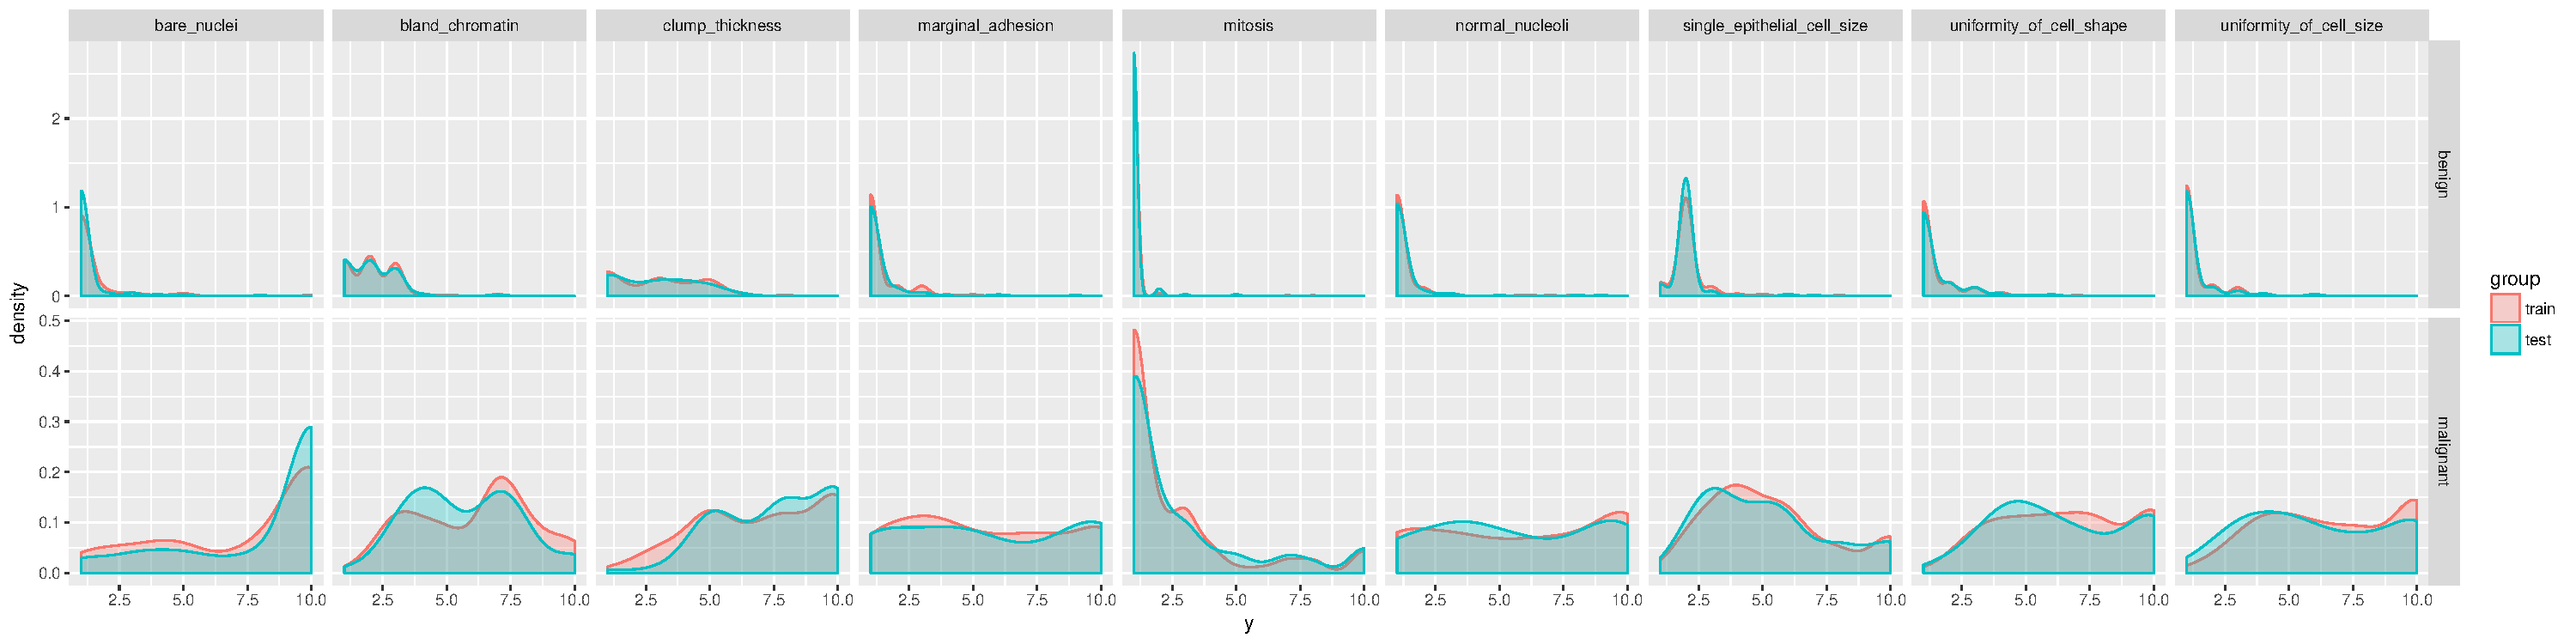
\includegraphics{webinar_code_files/figure-latex/unnamed-chunk-6-1} \end{center}

\paragraph{Classification}\label{classification}

\subparagraph{Decision trees}\label{decision-trees}

\begin{Shaded}
\begin{Highlighting}[]
\KeywordTok{library}\NormalTok{(rpart)}
\KeywordTok{library}\NormalTok{(rpart.plot)}

\KeywordTok{set.seed}\NormalTok{(}\DecValTok{42}\NormalTok{)}
\NormalTok{fit <-}\StringTok{ }\KeywordTok{rpart}\NormalTok{(classes ~}\StringTok{ }\NormalTok{.,}
            \DataTypeTok{data =} \NormalTok{train_data,}
            \DataTypeTok{method =} \StringTok{"class"}\NormalTok{,}
            \DataTypeTok{control =} \KeywordTok{rpart.control}\NormalTok{(}\DataTypeTok{xval =} \DecValTok{10}\NormalTok{, }
                                    \DataTypeTok{minbucket =} \DecValTok{2}\NormalTok{, }
                                    \DataTypeTok{cp =} \DecValTok{0}\NormalTok{), }
             \DataTypeTok{parms =} \KeywordTok{list}\NormalTok{(}\DataTypeTok{split =} \StringTok{"information"}\NormalTok{))}

\KeywordTok{rpart.plot}\NormalTok{(fit, }\DataTypeTok{extra =} \DecValTok{100}\NormalTok{)}
\end{Highlighting}
\end{Shaded}

\begin{center}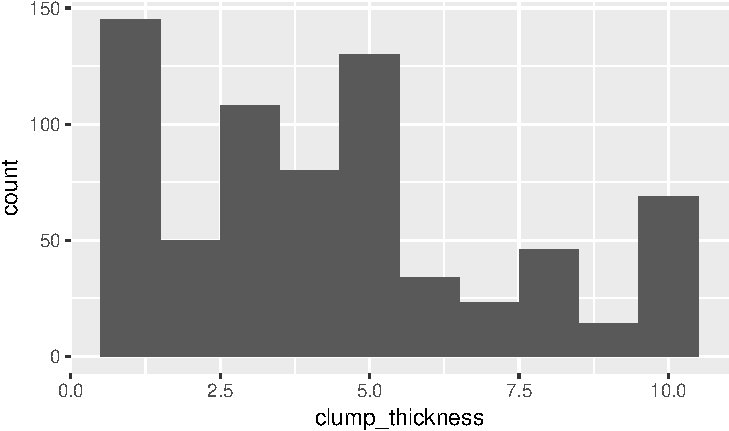
\includegraphics{webinar_code_files/figure-latex/unnamed-chunk-7-1} \end{center}

\subparagraph{Random Forests}\label{random-forests}

Can be used for classification and regression tasks. Here, I show a
classification task.

\begin{Shaded}
\begin{Highlighting}[]
\KeywordTok{set.seed}\NormalTok{(}\DecValTok{42}\NormalTok{)}
\NormalTok{model_rf <-}\StringTok{ }\NormalTok{caret::}\KeywordTok{train}\NormalTok{(classes ~}\StringTok{ }\NormalTok{.,}
                         \DataTypeTok{data =} \NormalTok{train_data,}
                         \DataTypeTok{method =} \StringTok{"rf"}\NormalTok{,}
                         \DataTypeTok{preProcess =} \KeywordTok{c}\NormalTok{(}\StringTok{"scale"}\NormalTok{, }\StringTok{"center"}\NormalTok{),}
                         \DataTypeTok{trControl =} \KeywordTok{trainControl}\NormalTok{(}\DataTypeTok{method =} \StringTok{"repeatedcv"}\NormalTok{, }
                                                  \DataTypeTok{number =} \DecValTok{10}\NormalTok{, }
                                                  \DataTypeTok{repeats =} \DecValTok{10}\NormalTok{, }
                                                  \DataTypeTok{savePredictions =} \OtherTok{TRUE}\NormalTok{, }
                                                  \DataTypeTok{verboseIter =} \OtherTok{FALSE}\NormalTok{))}
\end{Highlighting}
\end{Shaded}

When you specify \texttt{savePredictions\ =\ TRUE}, you can access the
cross-validation resuls with \texttt{model\_rf\$pred}.

\begin{itemize}
\tightlist
\item
  Feature Importance
\end{itemize}

\begin{Shaded}
\begin{Highlighting}[]
\CommentTok{# estimate variable importance}
\NormalTok{importance <-}\StringTok{ }\KeywordTok{varImp}\NormalTok{(model_rf, }\DataTypeTok{scale =} \OtherTok{TRUE}\NormalTok{)}

\KeywordTok{plot}\NormalTok{(importance)}
\end{Highlighting}
\end{Shaded}

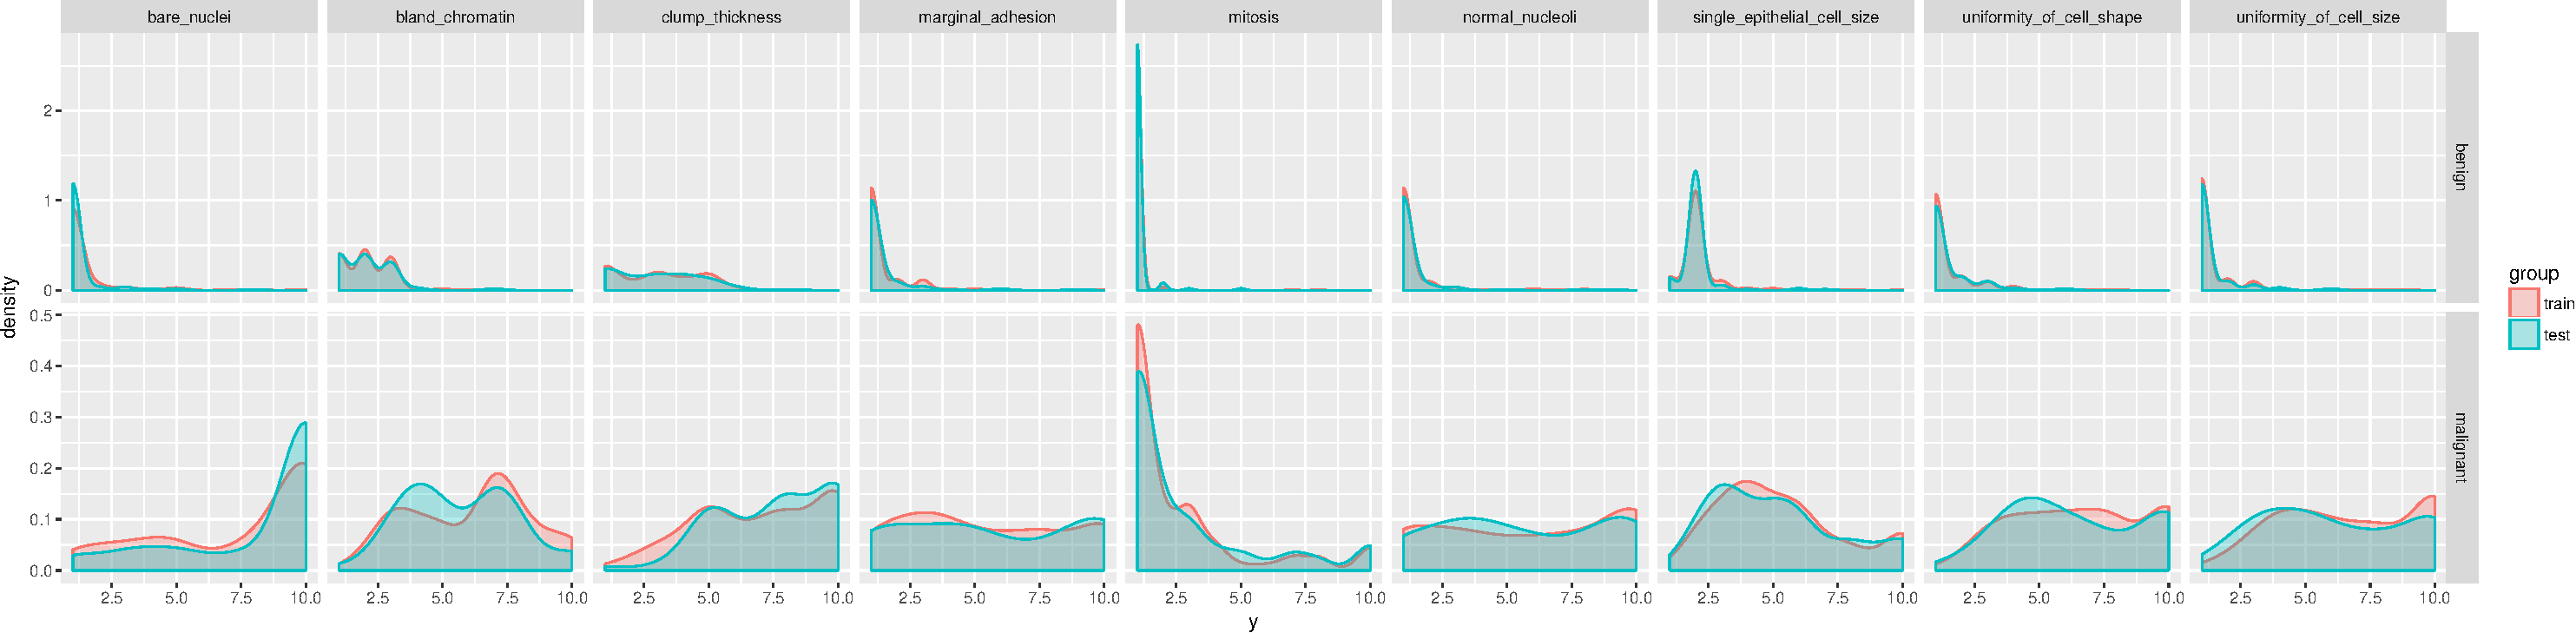
\includegraphics{webinar_code_files/figure-latex/unnamed-chunk-11-1.pdf}

\begin{itemize}
\tightlist
\item
  predicting test data
\end{itemize}

\begin{Shaded}
\begin{Highlighting}[]
\KeywordTok{confusionMatrix}\NormalTok{(}\KeywordTok{predict}\NormalTok{(model_rf, test_data), test_data$classes)}
\end{Highlighting}
\end{Shaded}

\begin{verbatim}
## Confusion Matrix and Statistics
## 
##            Reference
## Prediction  benign malignant
##   benign       133         2
##   malignant      4        70
##                                           
##                Accuracy : 0.9713          
##                  95% CI : (0.9386, 0.9894)
##     No Information Rate : 0.6555          
##     P-Value [Acc > NIR] : <2e-16          
##                                           
##                   Kappa : 0.9369          
##  Mcnemar's Test P-Value : 0.6831          
##                                           
##             Sensitivity : 0.9708          
##             Specificity : 0.9722          
##          Pos Pred Value : 0.9852          
##          Neg Pred Value : 0.9459          
##              Prevalence : 0.6555          
##          Detection Rate : 0.6364          
##    Detection Prevalence : 0.6459          
##       Balanced Accuracy : 0.9715          
##                                           
##        'Positive' Class : benign          
## 
\end{verbatim}

\subparagraph{Extreme gradient boosting
trees}\label{extreme-gradient-boosting-trees}

Can be used for classification and regression tasks. Here, I show a
classification task.

\begin{Shaded}
\begin{Highlighting}[]
\KeywordTok{set.seed}\NormalTok{(}\DecValTok{42}\NormalTok{)}
\NormalTok{model_xgb <-}\StringTok{ }\NormalTok{caret::}\KeywordTok{train}\NormalTok{(classes ~}\StringTok{ }\NormalTok{.,}
                          \DataTypeTok{data =} \NormalTok{train_data,}
                          \DataTypeTok{method =} \StringTok{"xgbTree"}\NormalTok{,}
                          \DataTypeTok{preProcess =} \KeywordTok{c}\NormalTok{(}\StringTok{"scale"}\NormalTok{, }\StringTok{"center"}\NormalTok{),}
                          \DataTypeTok{trControl =} \KeywordTok{trainControl}\NormalTok{(}\DataTypeTok{method =} \StringTok{"repeatedcv"}\NormalTok{, }
                                                  \DataTypeTok{number =} \DecValTok{10}\NormalTok{, }
                                                  \DataTypeTok{repeats =} \DecValTok{10}\NormalTok{, }
                                                  \DataTypeTok{savePredictions =} \OtherTok{TRUE}\NormalTok{, }
                                                  \DataTypeTok{verboseIter =} \OtherTok{FALSE}\NormalTok{))}
\end{Highlighting}
\end{Shaded}

\begin{itemize}
\tightlist
\item
  Feature Importance
\end{itemize}

\begin{Shaded}
\begin{Highlighting}[]
\CommentTok{# estimate variable importance}
\NormalTok{importance <-}\StringTok{ }\KeywordTok{varImp}\NormalTok{(model_xgb, }\DataTypeTok{scale =} \OtherTok{TRUE}\NormalTok{)}

\KeywordTok{plot}\NormalTok{(importance)}
\end{Highlighting}
\end{Shaded}

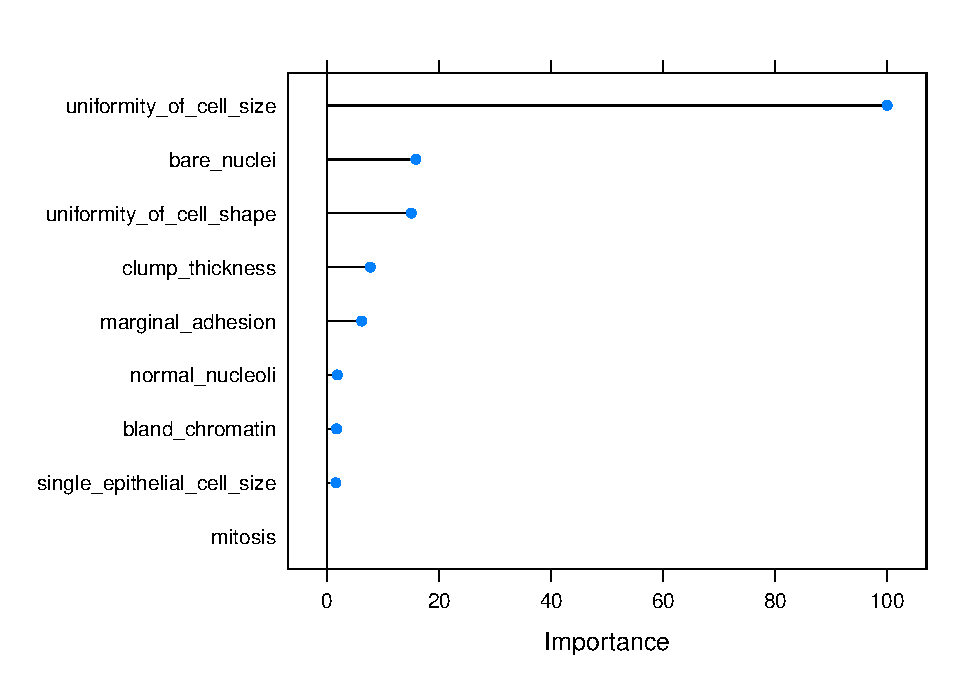
\includegraphics{webinar_code_files/figure-latex/unnamed-chunk-16-1.pdf}

\begin{itemize}
\tightlist
\item
  predicting test data
\end{itemize}

\begin{Shaded}
\begin{Highlighting}[]
\KeywordTok{confusionMatrix}\NormalTok{(}\KeywordTok{predict}\NormalTok{(model_xgb, test_data), test_data$classes)}
\end{Highlighting}
\end{Shaded}

\begin{verbatim}
## Confusion Matrix and Statistics
## 
##            Reference
## Prediction  benign malignant
##   benign       132         2
##   malignant      5        70
##                                           
##                Accuracy : 0.9665          
##                  95% CI : (0.9322, 0.9864)
##     No Information Rate : 0.6555          
##     P-Value [Acc > NIR] : <2e-16          
##                                           
##                   Kappa : 0.9266          
##  Mcnemar's Test P-Value : 0.4497          
##                                           
##             Sensitivity : 0.9635          
##             Specificity : 0.9722          
##          Pos Pred Value : 0.9851          
##          Neg Pred Value : 0.9333          
##              Prevalence : 0.6555          
##          Detection Rate : 0.6316          
##    Detection Prevalence : 0.6411          
##       Balanced Accuracy : 0.9679          
##                                           
##        'Positive' Class : benign          
## 
\end{verbatim}

\paragraph{Regression}\label{regression}

\begin{Shaded}
\begin{Highlighting}[]
\KeywordTok{set.seed}\NormalTok{(}\DecValTok{42}\NormalTok{)}
\NormalTok{model_glm <-}\StringTok{ }\NormalTok{caret::}\KeywordTok{train}\NormalTok{(clump_thickness ~}\StringTok{ }\NormalTok{.,}
                          \DataTypeTok{data =} \NormalTok{train_data,}
                          \DataTypeTok{method =} \StringTok{"glm"}\NormalTok{,}
                          \DataTypeTok{preProcess =} \KeywordTok{c}\NormalTok{(}\StringTok{"scale"}\NormalTok{, }\StringTok{"center"}\NormalTok{),}
                          \DataTypeTok{trControl =} \KeywordTok{trainControl}\NormalTok{(}\DataTypeTok{method =} \StringTok{"repeatedcv"}\NormalTok{, }
                                                  \DataTypeTok{number =} \DecValTok{10}\NormalTok{, }
                                                  \DataTypeTok{repeats =} \DecValTok{10}\NormalTok{, }
                                                  \DataTypeTok{savePredictions =} \OtherTok{TRUE}\NormalTok{, }
                                                  \DataTypeTok{verboseIter =} \OtherTok{FALSE}\NormalTok{))}
\end{Highlighting}
\end{Shaded}

\begin{Shaded}
\begin{Highlighting}[]
\KeywordTok{data.frame}\NormalTok{(}\DataTypeTok{actual =} \NormalTok{test_data$clump_thickness,}
           \DataTypeTok{predicted =} \KeywordTok{predict}\NormalTok{(model_glm, test_data)) %>%}
\StringTok{  }\KeywordTok{ggplot}\NormalTok{(}\KeywordTok{aes}\NormalTok{(}\DataTypeTok{x =} \NormalTok{actual, }\DataTypeTok{y =} \NormalTok{predicted)) +}
\StringTok{    }\KeywordTok{geom_jitter}\NormalTok{() +}
\StringTok{    }\KeywordTok{geom_smooth}\NormalTok{(}\DataTypeTok{method =} \StringTok{"lm"}\NormalTok{)}
\end{Highlighting}
\end{Shaded}

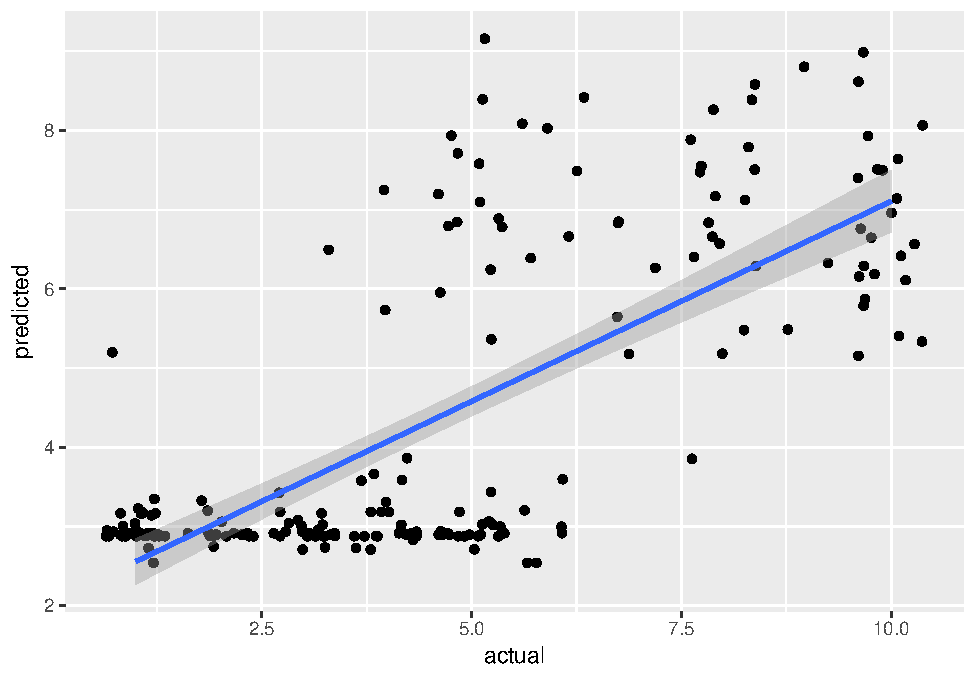
\includegraphics{webinar_code_files/figure-latex/unnamed-chunk-21-1.pdf}

\subsubsection{Grid search with h2o}\label{grid-search-with-h2o}

\begin{Shaded}
\begin{Highlighting}[]
\KeywordTok{library}\NormalTok{(h2o)}
\KeywordTok{h2o.init}\NormalTok{()}
\end{Highlighting}
\end{Shaded}

\begin{verbatim}
##  Connection successful!
## 
## R is connected to the H2O cluster: 
##     H2O cluster uptime:         21 minutes 15 seconds 
##     H2O cluster version:        3.10.3.6 
##     H2O cluster version age:    13 days  
##     H2O cluster name:           H2O_started_from_R_s_glan02_tbd690 
##     H2O cluster total nodes:    1 
##     H2O cluster total memory:   3.40 GB 
##     H2O cluster total cores:    8 
##     H2O cluster allowed cores:  2 
##     H2O cluster healthy:        TRUE 
##     H2O Connection ip:          localhost 
##     H2O Connection port:        54321 
##     H2O Connection proxy:       NA 
##     R Version:                  R version 3.3.2 (2016-10-31)
\end{verbatim}

\begin{Shaded}
\begin{Highlighting}[]
\NormalTok{bc_data_hf <-}\StringTok{ }\KeywordTok{as.h2o}\NormalTok{(bc_data)}
\end{Highlighting}
\end{Shaded}

\begin{verbatim}
## 
  |                                                                       
  |                                                                 |   0%
  |                                                                       
  |=================================================================| 100%
\end{verbatim}

\begin{Shaded}
\begin{Highlighting}[]
\KeywordTok{library}\NormalTok{(tidyr)}

\KeywordTok{h2o.describe}\NormalTok{(bc_data_hf) %>%}
\StringTok{  }\KeywordTok{gather}\NormalTok{(x, y, Zeros:Sigma) %>%}
\StringTok{  }\KeywordTok{mutate}\NormalTok{(}\DataTypeTok{group =} \KeywordTok{ifelse}\NormalTok{(x %in%}\StringTok{ }\KeywordTok{c}\NormalTok{(}\StringTok{"Min"}\NormalTok{, }\StringTok{"Max"}\NormalTok{, }\StringTok{"Mean"}\NormalTok{), }\StringTok{"min, mean, max"}\NormalTok{, }
                        \KeywordTok{ifelse}\NormalTok{(x %in%}\StringTok{ }\KeywordTok{c}\NormalTok{(}\StringTok{"NegInf"}\NormalTok{, }\StringTok{"PosInf"}\NormalTok{), }\StringTok{"Inf"}\NormalTok{, }\StringTok{"sigma, zeros"}\NormalTok{))) %>%}\StringTok{ }
\StringTok{  }\KeywordTok{ggplot}\NormalTok{(}\KeywordTok{aes}\NormalTok{(}\DataTypeTok{x =} \NormalTok{Label, }\DataTypeTok{y =} \KeywordTok{as.numeric}\NormalTok{(y), }\DataTypeTok{color =} \NormalTok{x)) +}
\StringTok{    }\KeywordTok{geom_point}\NormalTok{(}\DataTypeTok{size =} \DecValTok{4}\NormalTok{, }\DataTypeTok{alpha =} \FloatTok{0.6}\NormalTok{) +}
\StringTok{    }\KeywordTok{scale_color_brewer}\NormalTok{(}\DataTypeTok{palette =} \StringTok{"Set1"}\NormalTok{) +}
\StringTok{    }\KeywordTok{theme}\NormalTok{(}\DataTypeTok{axis.text.x =} \KeywordTok{element_text}\NormalTok{(}\DataTypeTok{angle =} \DecValTok{45}\NormalTok{, }\DataTypeTok{vjust =} \DecValTok{1}\NormalTok{, }\DataTypeTok{hjust =} \DecValTok{1}\NormalTok{)) +}
\StringTok{    }\KeywordTok{facet_grid}\NormalTok{(group ~}\StringTok{ }\NormalTok{., }\DataTypeTok{scales =} \StringTok{"free"}\NormalTok{) +}
\StringTok{    }\KeywordTok{labs}\NormalTok{(}\DataTypeTok{x =} \StringTok{"Feature"}\NormalTok{,}
         \DataTypeTok{y =} \StringTok{"Value"}\NormalTok{,}
         \DataTypeTok{color =} \StringTok{""}\NormalTok{)}
\end{Highlighting}
\end{Shaded}

\begin{center}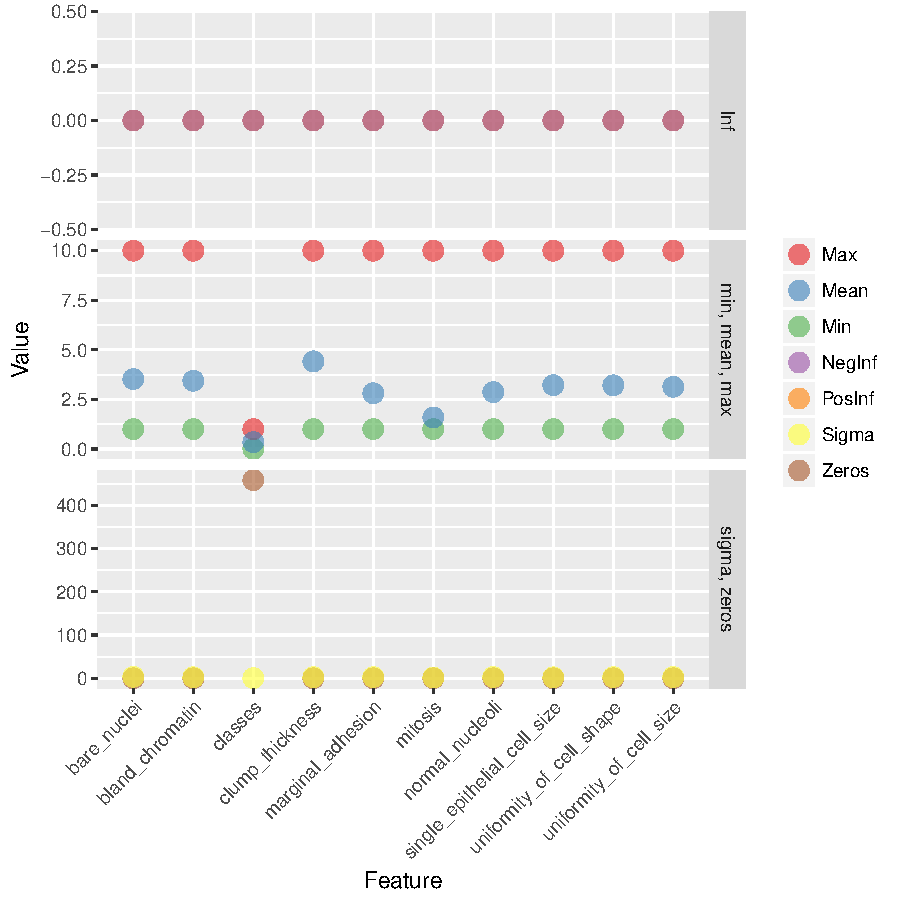
\includegraphics{webinar_code_files/figure-latex/unnamed-chunk-23-1} \end{center}

\paragraph{Training, validation and test
data}\label{training-validation-and-test-data-1}

\begin{Shaded}
\begin{Highlighting}[]
\NormalTok{splits <-}\StringTok{ }\KeywordTok{h2o.splitFrame}\NormalTok{(bc_data_hf, }
                         \DataTypeTok{ratios =} \KeywordTok{c}\NormalTok{(}\FloatTok{0.7}\NormalTok{, }\FloatTok{0.15}\NormalTok{), }
                         \DataTypeTok{seed =} \DecValTok{1}\NormalTok{)}

\NormalTok{train <-}\StringTok{ }\NormalTok{splits[[}\DecValTok{1}\NormalTok{]]}
\NormalTok{valid <-}\StringTok{ }\NormalTok{splits[[}\DecValTok{2}\NormalTok{]]}
\NormalTok{test <-}\StringTok{ }\NormalTok{splits[[}\DecValTok{3}\NormalTok{]]}

\NormalTok{response <-}\StringTok{ "classes"}
\NormalTok{features <-}\StringTok{ }\KeywordTok{setdiff}\NormalTok{(}\KeywordTok{colnames}\NormalTok{(train), response)}
\end{Highlighting}
\end{Shaded}

\begin{Shaded}
\begin{Highlighting}[]
\KeywordTok{summary}\NormalTok{(train$classes, }\DataTypeTok{exact_quantiles =} \OtherTok{TRUE}\NormalTok{)}
\end{Highlighting}
\end{Shaded}

\begin{verbatim}
##  classes       
##  benign   :317 
##  malignant:174
\end{verbatim}

\begin{Shaded}
\begin{Highlighting}[]
\KeywordTok{summary}\NormalTok{(valid$classes, }\DataTypeTok{exact_quantiles =} \OtherTok{TRUE}\NormalTok{)}
\end{Highlighting}
\end{Shaded}

\begin{verbatim}
##  classes      
##  benign   :71 
##  malignant:35
\end{verbatim}

\begin{Shaded}
\begin{Highlighting}[]
\KeywordTok{summary}\NormalTok{(test$classes, }\DataTypeTok{exact_quantiles =} \OtherTok{TRUE}\NormalTok{)}
\end{Highlighting}
\end{Shaded}

\begin{verbatim}
##  classes      
##  benign   :70 
##  malignant:32
\end{verbatim}

\paragraph{Classification}\label{classification-1}

\subparagraph{Random Forest}\label{random-forest}

Can be used for classification and regression tasks. Here, I show a
classification task.

\begin{Shaded}
\begin{Highlighting}[]
\NormalTok{hyper_params <-}\StringTok{ }\KeywordTok{list}\NormalTok{(}
                     \DataTypeTok{ntrees =} \KeywordTok{c}\NormalTok{(}\DecValTok{25}\NormalTok{, }\DecValTok{50}\NormalTok{, }\DecValTok{75}\NormalTok{, }\DecValTok{100}\NormalTok{),}
                     \DataTypeTok{max_depth =} \KeywordTok{c}\NormalTok{(}\DecValTok{10}\NormalTok{, }\DecValTok{20}\NormalTok{, }\DecValTok{30}\NormalTok{),}
                     \DataTypeTok{min_rows =} \KeywordTok{c}\NormalTok{(}\DecValTok{1}\NormalTok{, }\DecValTok{3}\NormalTok{, }\DecValTok{5}\NormalTok{)}
                     \NormalTok{)}

\NormalTok{search_criteria <-}\StringTok{ }\KeywordTok{list}\NormalTok{(}
                        \DataTypeTok{strategy =} \StringTok{"RandomDiscrete"}\NormalTok{, }
                        \DataTypeTok{max_models =} \DecValTok{50}\NormalTok{,}
                        \DataTypeTok{max_runtime_secs =} \DecValTok{360}\NormalTok{,}
                        \DataTypeTok{stopping_rounds =} \DecValTok{5}\NormalTok{,          }
                        \DataTypeTok{stopping_metric =} \StringTok{"AUC"}\NormalTok{,      }
                        \DataTypeTok{stopping_tolerance =} \FloatTok{0.0005}\NormalTok{,}
                        \DataTypeTok{seed =} \DecValTok{42}
                        \NormalTok{)}
\end{Highlighting}
\end{Shaded}

\begin{Shaded}
\begin{Highlighting}[]
\NormalTok{rf_grid <-}\StringTok{ }\KeywordTok{h2o.grid}\NormalTok{(}\DataTypeTok{algorithm =} \StringTok{"randomForest"}\NormalTok{, }\CommentTok{# h2o.randomForest, }
                                                \CommentTok{# alternatively h2o.gbm for Gradient boosting trees}
                    \DataTypeTok{x =} \NormalTok{features,}
                    \DataTypeTok{y =} \NormalTok{response,}
                    \DataTypeTok{grid_id =} \StringTok{"rf_grid"}\NormalTok{,}
                    \DataTypeTok{training_frame =} \NormalTok{train,}
                    \DataTypeTok{validation_frame =} \NormalTok{valid,}
                    \DataTypeTok{nfolds =} \DecValTok{25}\NormalTok{,                           }
                    \DataTypeTok{fold_assignment =} \StringTok{"Stratified"}\NormalTok{,}
                    \DataTypeTok{hyper_params =} \NormalTok{hyper_params,}
                    \DataTypeTok{search_criteria =} \NormalTok{search_criteria,}
                    \DataTypeTok{seed =} \DecValTok{42}
                    \NormalTok{)}
\end{Highlighting}
\end{Shaded}

\begin{Shaded}
\begin{Highlighting}[]
\CommentTok{# performance metrics where smaller is better -> order with decreasing = FALSE}
\NormalTok{sort_options_1 <-}\StringTok{ }\KeywordTok{c}\NormalTok{(}\StringTok{"mean_per_class_error"}\NormalTok{, }\StringTok{"mse"}\NormalTok{, }\StringTok{"err"}\NormalTok{, }\StringTok{"logloss"}\NormalTok{)}

\NormalTok{for (sort_by_1 in sort_options_1) \{}
  
  \NormalTok{grid <-}\StringTok{ }\KeywordTok{h2o.getGrid}\NormalTok{(}\StringTok{"rf_grid"}\NormalTok{, }\DataTypeTok{sort_by =} \NormalTok{sort_by_1, }\DataTypeTok{decreasing =} \OtherTok{FALSE}\NormalTok{)}
  
  \NormalTok{model_ids <-}\StringTok{ }\NormalTok{grid@model_ids}
  \NormalTok{best_model <-}\StringTok{ }\KeywordTok{h2o.getModel}\NormalTok{(model_ids[[}\DecValTok{1}\NormalTok{]])}
  
  \KeywordTok{h2o.saveModel}\NormalTok{(best_model, }\DataTypeTok{path=}\StringTok{"models"}\NormalTok{, }\DataTypeTok{force =} \OtherTok{TRUE}\NormalTok{)}
  
\NormalTok{\}}


\CommentTok{# performance metrics where bigger is better -> order with decreasing = TRUE}
\NormalTok{sort_options_2 <-}\StringTok{ }\KeywordTok{c}\NormalTok{(}\StringTok{"auc"}\NormalTok{, }\StringTok{"precision"}\NormalTok{, }\StringTok{"accuracy"}\NormalTok{, }\StringTok{"recall"}\NormalTok{, }\StringTok{"specificity"}\NormalTok{)}

\NormalTok{for (sort_by_2 in sort_options_2) \{}
  
  \NormalTok{grid <-}\StringTok{ }\KeywordTok{h2o.getGrid}\NormalTok{(}\StringTok{"rf_grid"}\NormalTok{, }\DataTypeTok{sort_by =} \NormalTok{sort_by_2, }\DataTypeTok{decreasing =} \OtherTok{TRUE}\NormalTok{)}
  
  \NormalTok{model_ids <-}\StringTok{ }\NormalTok{grid@model_ids}
  \NormalTok{best_model <-}\StringTok{ }\KeywordTok{h2o.getModel}\NormalTok{(model_ids[[}\DecValTok{1}\NormalTok{]])}
  
  \KeywordTok{h2o.saveModel}\NormalTok{(best_model, }\DataTypeTok{path=}\StringTok{"models"}\NormalTok{, }\DataTypeTok{force =} \OtherTok{TRUE}\NormalTok{)}
  
\NormalTok{\}}
\end{Highlighting}
\end{Shaded}

\begin{Shaded}
\begin{Highlighting}[]
\NormalTok{files <-}\StringTok{ }\KeywordTok{list.files}\NormalTok{(}\DataTypeTok{path =} \StringTok{"models"}\NormalTok{)}
\NormalTok{rf_models <-}\StringTok{ }\NormalTok{files[}\KeywordTok{grep}\NormalTok{(}\StringTok{"rf_grid_model"}\NormalTok{, files)]}

\NormalTok{for (model_id in rf_models) \{}
  
  \NormalTok{path <-}\StringTok{ }\KeywordTok{paste0}\NormalTok{(}\StringTok{"U:}\CharTok{\textbackslash{}\textbackslash{}}\StringTok{Github_blog}\CharTok{\textbackslash{}\textbackslash{}}\StringTok{Webinar}\CharTok{\textbackslash{}\textbackslash{}}\StringTok{Webinar_ML_for_disease}\CharTok{\textbackslash{}\textbackslash{}}\StringTok{models}\CharTok{\textbackslash{}\textbackslash{}}\StringTok{"}\NormalTok{, model_id)}
  \NormalTok{best_model <-}\StringTok{ }\KeywordTok{h2o.loadModel}\NormalTok{(path)}
  \NormalTok{mse_auc_test <-}\StringTok{ }\KeywordTok{data.frame}\NormalTok{(}\DataTypeTok{model_id =} \NormalTok{model_id, }
                             \DataTypeTok{mse =} \KeywordTok{h2o.mse}\NormalTok{(}\KeywordTok{h2o.performance}\NormalTok{(best_model, test)),}
                             \DataTypeTok{auc =} \KeywordTok{h2o.auc}\NormalTok{(}\KeywordTok{h2o.performance}\NormalTok{(best_model, test)))}
  
  \NormalTok{if (model_id ==}\StringTok{ }\NormalTok{rf_models[[}\DecValTok{1}\NormalTok{]]) \{}
    
    \NormalTok{mse_auc_test_comb <-}\StringTok{ }\NormalTok{mse_auc_test}
    
  \NormalTok{\} else \{}
    
    \NormalTok{mse_auc_test_comb <-}\StringTok{ }\KeywordTok{rbind}\NormalTok{(mse_auc_test_comb, mse_auc_test)}
    
  \NormalTok{\}}
\NormalTok{\}}

\NormalTok{mse_auc_test_comb %>%}
\StringTok{  }\KeywordTok{gather}\NormalTok{(x, y, mse:auc) %>%}
\StringTok{  }\KeywordTok{ggplot}\NormalTok{(}\KeywordTok{aes}\NormalTok{(}\DataTypeTok{x =} \NormalTok{model_id, }\DataTypeTok{y =} \NormalTok{y, }\DataTypeTok{fill =} \NormalTok{model_id)) +}
\StringTok{    }\KeywordTok{facet_grid}\NormalTok{(x ~}\StringTok{ }\NormalTok{., }\DataTypeTok{scales =} \StringTok{"free"}\NormalTok{) +}
\StringTok{    }\KeywordTok{geom_bar}\NormalTok{(}\DataTypeTok{stat =} \StringTok{"identity"}\NormalTok{, }\DataTypeTok{alpha =} \FloatTok{0.8}\NormalTok{, }\DataTypeTok{position =} \StringTok{"dodge"}\NormalTok{) +}
\StringTok{    }\KeywordTok{scale_fill_brewer}\NormalTok{(}\DataTypeTok{palette =} \StringTok{"Set1"}\NormalTok{) +}
\StringTok{    }\KeywordTok{theme}\NormalTok{(}\DataTypeTok{axis.text.x =} \KeywordTok{element_text}\NormalTok{(}\DataTypeTok{angle =} \DecValTok{45}\NormalTok{, }\DataTypeTok{vjust =} \DecValTok{1}\NormalTok{, }\DataTypeTok{hjust=}\DecValTok{1}\NormalTok{),}
          \DataTypeTok{plot.margin =} \KeywordTok{unit}\NormalTok{(}\KeywordTok{c}\NormalTok{(}\FloatTok{0.5}\NormalTok{, }\DecValTok{0}\NormalTok{, }\DecValTok{0}\NormalTok{, }\FloatTok{1.5}\NormalTok{), }\StringTok{"cm"}\NormalTok{)) +}
\StringTok{    }\KeywordTok{labs}\NormalTok{(}\DataTypeTok{x =} \StringTok{""}\NormalTok{, }\DataTypeTok{y =} \StringTok{"value"}\NormalTok{, }\DataTypeTok{fill =} \StringTok{""}\NormalTok{)}
\end{Highlighting}
\end{Shaded}

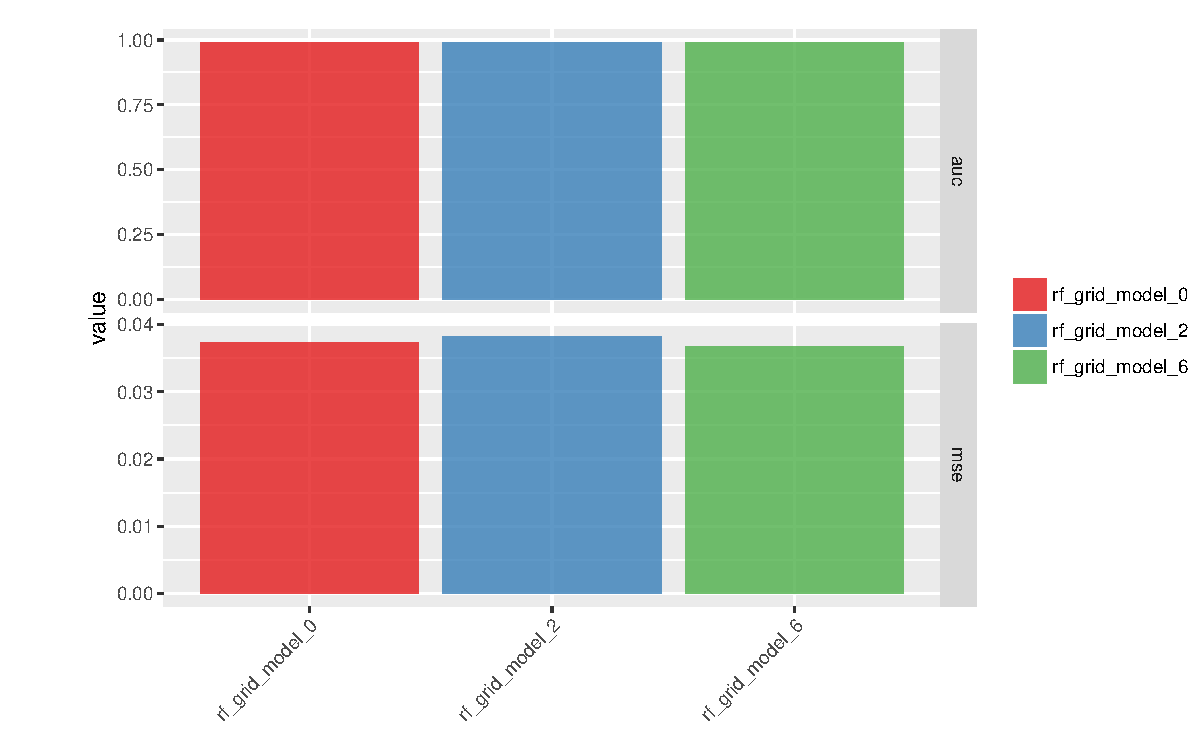
\includegraphics{webinar_code_files/figure-latex/unnamed-chunk-29-1.pdf}

\begin{Shaded}
\begin{Highlighting}[]
\NormalTok{for (model_id in rf_models) \{}
  
  \NormalTok{best_model <-}\StringTok{ }\KeywordTok{h2o.getModel}\NormalTok{(model_id)}
  
  \NormalTok{finalRf_predictions <-}\StringTok{ }\KeywordTok{data.frame}\NormalTok{(}\DataTypeTok{model_id =} \KeywordTok{rep}\NormalTok{(best_model@model_id, }
                                                   \KeywordTok{nrow}\NormalTok{(test)),}
                                    \DataTypeTok{actual =} \KeywordTok{as.vector}\NormalTok{(test$classes), }
                                    \KeywordTok{as.data.frame}\NormalTok{(}\KeywordTok{h2o.predict}\NormalTok{(}\DataTypeTok{object =} \NormalTok{best_model, }
                                                              \DataTypeTok{newdata =} \NormalTok{test)))}
  
  \NormalTok{finalRf_predictions$accurate <-}\StringTok{ }\KeywordTok{ifelse}\NormalTok{(finalRf_predictions$actual ==}\StringTok{ }\NormalTok{finalRf_predictions$predict, }
                                         \StringTok{"yes"}\NormalTok{, }\StringTok{"no"}\NormalTok{)}
  
  \NormalTok{finalRf_predictions$predict_stringent <-}\StringTok{ }\KeywordTok{ifelse}\NormalTok{(finalRf_predictions$benign >}\StringTok{ }\FloatTok{0.8}\NormalTok{, }
                                                  \StringTok{"benign"}\NormalTok{, }
                                                  \KeywordTok{ifelse}\NormalTok{(finalRf_predictions$malignant >}\StringTok{ }\FloatTok{0.8}\NormalTok{, }
                                                         \StringTok{"malignant"}\NormalTok{, }\StringTok{"uncertain"}\NormalTok{))}
  
  \NormalTok{finalRf_predictions$accurate_stringent <-}\StringTok{ }\KeywordTok{ifelse}\NormalTok{(finalRf_predictions$actual ==}\StringTok{ }\NormalTok{finalRf_predictions$predict_stringent, }
                                                   \StringTok{"yes"}\NormalTok{, }
                                         \KeywordTok{ifelse}\NormalTok{(finalRf_predictions$predict_stringent ==}\StringTok{ "uncertain"}\NormalTok{, }
                                                \StringTok{"na"}\NormalTok{, }\StringTok{"no"}\NormalTok{))}
  
  \NormalTok{if (model_id ==}\StringTok{ }\NormalTok{rf_models[[}\DecValTok{1}\NormalTok{]]) \{}
    
    \NormalTok{finalRf_predictions_comb <-}\StringTok{ }\NormalTok{finalRf_predictions}
    
  \NormalTok{\} else \{}
    
    \NormalTok{finalRf_predictions_comb <-}\StringTok{ }\KeywordTok{rbind}\NormalTok{(finalRf_predictions_comb, finalRf_predictions)}
    
  \NormalTok{\}}
\NormalTok{\}}
\end{Highlighting}
\end{Shaded}

\begin{verbatim}
## 
  |                                                                       
  |                                                                 |   0%
  |                                                                       
  |=================================================================| 100%
## 
  |                                                                       
  |                                                                 |   0%
  |                                                                       
  |=================================================================| 100%
## 
  |                                                                       
  |                                                                 |   0%
  |                                                                       
  |=================================================================| 100%
\end{verbatim}

\begin{Shaded}
\begin{Highlighting}[]
\NormalTok{finalRf_predictions_comb %>%}
\StringTok{  }\KeywordTok{ggplot}\NormalTok{(}\KeywordTok{aes}\NormalTok{(}\DataTypeTok{x =} \NormalTok{actual, }\DataTypeTok{fill =} \NormalTok{accurate)) +}
\StringTok{    }\KeywordTok{geom_bar}\NormalTok{(}\DataTypeTok{position =} \StringTok{"dodge"}\NormalTok{) +}
\StringTok{    }\KeywordTok{scale_fill_brewer}\NormalTok{(}\DataTypeTok{palette =} \StringTok{"Set1"}\NormalTok{) +}
\StringTok{    }\KeywordTok{facet_wrap}\NormalTok{(~}\StringTok{ }\NormalTok{model_id, }\DataTypeTok{ncol =} \DecValTok{3}\NormalTok{) +}
\StringTok{    }\KeywordTok{labs}\NormalTok{(}\DataTypeTok{fill =} \StringTok{"Were}\CharTok{\textbackslash{}n}\StringTok{predictions}\CharTok{\textbackslash{}n}\StringTok{accurate?"}\NormalTok{,}
         \DataTypeTok{title =} \StringTok{"Default predictions"}\NormalTok{)}
\end{Highlighting}
\end{Shaded}

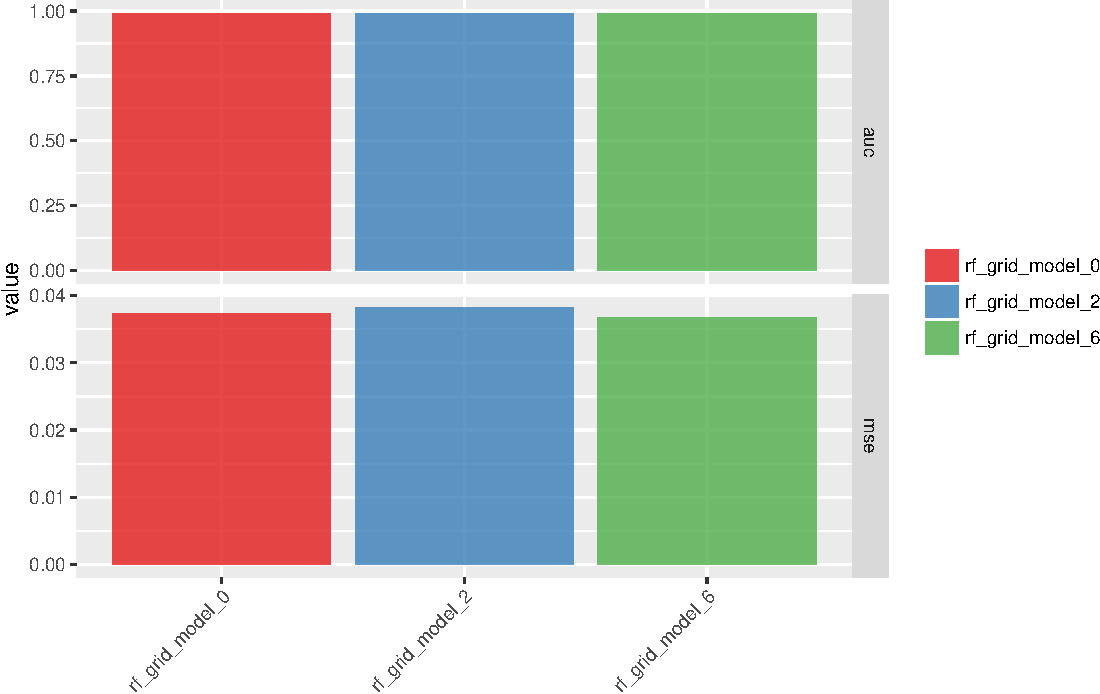
\includegraphics{webinar_code_files/figure-latex/unnamed-chunk-31-1.pdf}

\begin{Shaded}
\begin{Highlighting}[]
\NormalTok{finalRf_predictions_comb %>%}
\StringTok{  }\KeywordTok{subset}\NormalTok{(accurate_stringent !=}\StringTok{ "na"}\NormalTok{) %>%}
\StringTok{  }\KeywordTok{ggplot}\NormalTok{(}\KeywordTok{aes}\NormalTok{(}\DataTypeTok{x =} \NormalTok{actual, }\DataTypeTok{fill =} \NormalTok{accurate_stringent)) +}
\StringTok{    }\KeywordTok{geom_bar}\NormalTok{(}\DataTypeTok{position =} \StringTok{"dodge"}\NormalTok{) +}
\StringTok{    }\KeywordTok{scale_fill_brewer}\NormalTok{(}\DataTypeTok{palette =} \StringTok{"Set1"}\NormalTok{) +}
\StringTok{    }\KeywordTok{facet_wrap}\NormalTok{(~}\StringTok{ }\NormalTok{model_id, }\DataTypeTok{ncol =} \DecValTok{3}\NormalTok{) +}
\StringTok{    }\KeywordTok{labs}\NormalTok{(}\DataTypeTok{fill =} \StringTok{"Were}\CharTok{\textbackslash{}n}\StringTok{predictions}\CharTok{\textbackslash{}n}\StringTok{accurate?"}\NormalTok{,}
         \DataTypeTok{title =} \StringTok{"Stringent predictions"}\NormalTok{)}
\end{Highlighting}
\end{Shaded}

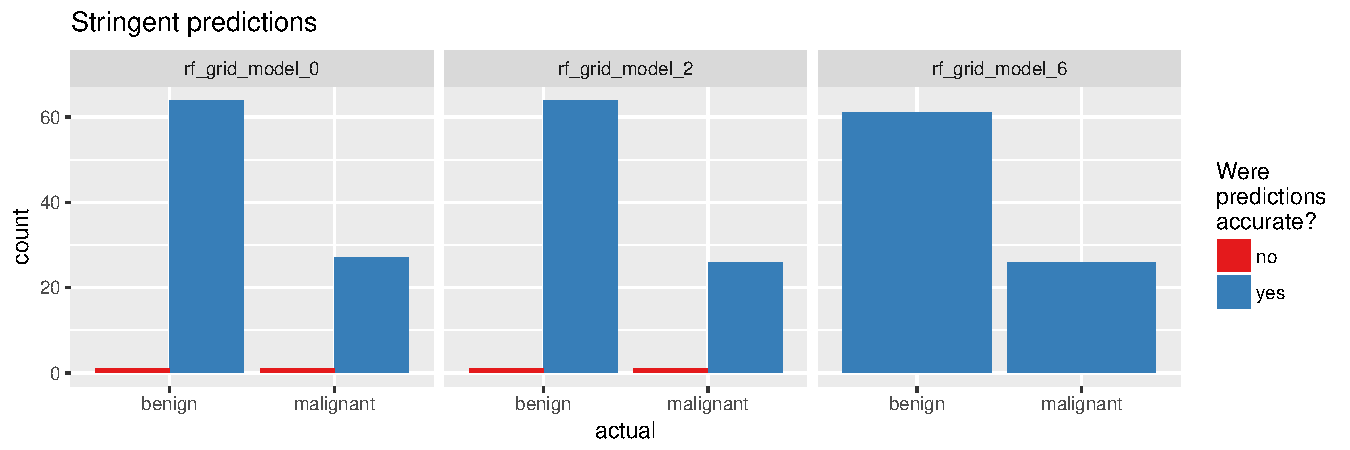
\includegraphics{webinar_code_files/figure-latex/unnamed-chunk-31-2.pdf}

\begin{Shaded}
\begin{Highlighting}[]
\NormalTok{rf_model <-}\StringTok{ }\KeywordTok{h2o.loadModel}\NormalTok{(}\StringTok{"U:}\CharTok{\textbackslash{}\textbackslash{}}\StringTok{Github_blog}\CharTok{\textbackslash{}\textbackslash{}}\StringTok{Webinar}\CharTok{\textbackslash{}\textbackslash{}}\StringTok{Webinar_ML_for_disease}\CharTok{\textbackslash{}\textbackslash{}}\StringTok{models}\CharTok{\textbackslash{}\textbackslash{}}\StringTok{rf_grid_model_6"}\NormalTok{)}
\NormalTok{rf_model}
\end{Highlighting}
\end{Shaded}

\begin{verbatim}
## Model Details:
## ==============
## 
## H2OBinomialModel: drf
## Model ID:  rf_grid_model_6 
## Model Summary: 
##   number_of_trees number_of_internal_trees model_size_in_bytes min_depth
## 1             100                      100               24848         4
##   max_depth mean_depth min_leaves max_leaves mean_leaves
## 1         9    5.77000          8         17    12.94000
## 
## 
## H2OBinomialMetrics: drf
## ** Reported on training data. **
## ** Metrics reported on Out-Of-Bag training samples **
## 
## MSE:  0.03055597
## RMSE:  0.1748027
## LogLoss:  0.1140213
## Mean Per-Class Error:  0.02467457
## AUC:  0.989521
## Gini:  0.979042
## 
## Confusion Matrix (vertical: actual; across: predicted) for F1-optimal threshold:
##           benign malignant    Error     Rate
## benign       305        12 0.037855  =12/317
## malignant      2       172 0.011494   =2/174
## Totals       307       184 0.028513  =14/491
## 
## Maximum Metrics: Maximum metrics at their respective thresholds
##                         metric threshold    value idx
## 1                       max f1  0.445310 0.960894 172
## 2                       max f2  0.214464 0.977528 182
## 3                 max f0point5  0.552688 0.946712 165
## 4                 max accuracy  0.445310 0.971487 172
## 5                max precision  1.000000 1.000000   0
## 6                   max recall  0.214464 1.000000 182
## 7              max specificity  1.000000 1.000000   0
## 8             max absolute_mcc  0.445310 0.939393 172
## 9   max min_per_class_accuracy  0.487375 0.965300 167
## 10 max mean_per_class_accuracy  0.445310 0.975325 172
## 
## Gains/Lift Table: Extract with `h2o.gainsLift(<model>, <data>)` or `h2o.gainsLift(<model>, valid=<T/F>, xval=<T/F>)`
## H2OBinomialMetrics: drf
## ** Reported on validation data. **
## 
## MSE:  0.01590167
## RMSE:  0.1261018
## LogLoss:  0.07067446
## Mean Per-Class Error:  0.007042254
## AUC:  0.9995976
## Gini:  0.9991952
## 
## Confusion Matrix (vertical: actual; across: predicted) for F1-optimal threshold:
##           benign malignant    Error    Rate
## benign        70         1 0.014085   =1/71
## malignant      0        35 0.000000   =0/35
## Totals        70        36 0.009434  =1/106
## 
## Maximum Metrics: Maximum metrics at their respective thresholds
##                         metric threshold    value idx
## 1                       max f1  0.293126 0.985915  34
## 2                       max f2  0.293126 0.994318  34
## 3                 max f0point5  0.555841 0.994152  32
## 4                 max accuracy  0.555841 0.990566  32
## 5                max precision  1.000000 1.000000   0
## 6                   max recall  0.293126 1.000000  34
## 7              max specificity  1.000000 1.000000   0
## 8             max absolute_mcc  0.293126 0.979045  34
## 9   max min_per_class_accuracy  0.293126 0.985915  34
## 10 max mean_per_class_accuracy  0.293126 0.992958  34
## 
## Gains/Lift Table: Extract with `h2o.gainsLift(<model>, <data>)` or `h2o.gainsLift(<model>, valid=<T/F>, xval=<T/F>)`
## H2OBinomialMetrics: drf
## ** Reported on cross-validation data. **
## ** 25-fold cross-validation on training data (Metrics computed for combined holdout predictions) **
## 
## MSE:  0.03141201
## RMSE:  0.1772343
## LogLoss:  0.1163767
## Mean Per-Class Error:  0.02309728
## AUC:  0.9890496
## Gini:  0.9780993
## 
## Confusion Matrix (vertical: actual; across: predicted) for F1-optimal threshold:
##           benign malignant    Error     Rate
## benign       306        11 0.034700  =11/317
## malignant      2       172 0.011494   =2/174
## Totals       308       183 0.026477  =13/491
## 
## Maximum Metrics: Maximum metrics at their respective thresholds
##                         metric threshold    value idx
## 1                       max f1  0.458037 0.963585 178
## 2                       max f2  0.458037 0.978385 178
## 3                 max f0point5  0.514579 0.952116 176
## 4                 max accuracy  0.514579 0.973523 176
## 5                max precision  1.000000 1.000000   0
## 6                   max recall  0.182569 1.000000 196
## 7              max specificity  1.000000 1.000000   0
## 8             max absolute_mcc  0.458037 0.943546 178
## 9   max min_per_class_accuracy  0.530369 0.968454 174
## 10 max mean_per_class_accuracy  0.458037 0.976903 178
## 
## Gains/Lift Table: Extract with `h2o.gainsLift(<model>, <data>)` or `h2o.gainsLift(<model>, valid=<T/F>, xval=<T/F>)`
## Cross-Validation Metrics Summary: 
##                                mean           sd  cv_1_valid  cv_2_valid
## accuracy                 0.97824687  0.022163384         1.0         1.0
## auc                      0.98896265 0.0137583455         1.0         1.0
## err                     0.021753136  0.022163384         0.0         0.0
## err_count                       0.4          0.4         0.0         0.0
## f0point5                 0.94340783  0.060686026         1.0         1.0
## f1                       0.96193475   0.04148564         1.0         1.0
## f2                        0.9834832   0.01836118         1.0         1.0
## lift_top_group             3.146508   0.86633277         3.0   2.6666667
## logloss                  0.12211874   0.06134508 0.051629476  0.09666276
## max_per_class_error     0.031400856  0.032273438         0.0         0.0
## mcc                       0.9496154  0.051578306         1.0         1.0
## mean_per_class_accuracy   0.9842996  0.016136719         1.0         1.0
## mean_per_class_error    0.015700428  0.016136719         0.0         0.0
## mse                     0.033157483   0.02053207 0.008940321 0.022683756
## precision                 0.9323954   0.07182843         1.0         1.0
## r2                        0.8243174    0.1447473  0.95976853  0.90321594
## recall                          1.0          0.0         1.0         1.0
## rmse                     0.16665597  0.051880974  0.09455328  0.15061128
## specificity              0.96859914  0.032273438         1.0         1.0
##                          cv_3_valid   cv_4_valid  cv_5_valid  cv_6_valid
## accuracy                 0.95454544          1.0         1.0   0.9285714
## auc                       0.9764706          1.0         1.0   0.9583333
## err                     0.045454547          0.0         0.0 0.071428575
## err_count                       1.0          0.0         0.0         1.0
## f0point5                 0.86206895          1.0         1.0  0.71428573
## f1                       0.90909094          1.0         1.0         0.8
## f2                       0.96153843          1.0         1.0  0.90909094
## lift_top_group                  4.4          2.5   2.7777777         7.0
## logloss                  0.14851098  0.032063406  0.07835095  0.38401476
## max_per_class_error      0.05882353          0.0         0.0 0.083333336
## mcc                       0.8856149          1.0         1.0  0.78173596
## mean_per_class_accuracy   0.9705882          1.0         1.0   0.9583333
## mean_per_class_error    0.029411765          0.0         0.0 0.041666668
## mse                     0.048121125 0.0026525913 0.017376833  0.12076553
## precision                 0.8333333          1.0         1.0   0.6666667
## r2                        0.7259927    0.9889475  0.92457974 0.013748176
## recall                          1.0          1.0         1.0         1.0
## rmse                     0.21936527  0.051503316  0.13182122  0.34751335
## specificity               0.9411765          1.0         1.0   0.9166667
##                          cv_7_valid  cv_8_valid  cv_9_valid cv_10_valid
## accuracy                 0.94736844   0.9411765   0.8888889         1.0
## auc                      0.98571426   0.9848485   0.9230769         1.0
## err                      0.05263158  0.05882353  0.11111111         0.0
## err_count                       1.0         1.0         2.0         0.0
## f0point5                 0.86206895  0.88235295  0.75757575         1.0
## f1                       0.90909094   0.9230769   0.8333333         1.0
## f2                       0.96153843   0.9677419   0.9259259         1.0
## lift_top_group                  3.8   2.8333333         3.6   1.7142857
## logloss                  0.12703204   0.1548704  0.36086315  0.10401911
## max_per_class_error     0.071428575  0.09090909  0.15384616         0.0
## mcc                       0.8796644  0.88273484  0.77742887         1.0
## mean_per_class_accuracy  0.96428573  0.95454544   0.9230769         1.0
## mean_per_class_error    0.035714287 0.045454547  0.07692308         0.0
## mse                      0.04287585 0.051242344 0.104545906 0.019419663
## precision                 0.8333333  0.85714287  0.71428573         1.0
## r2                       0.77888316  0.77562064  0.47887886  0.92010194
## recall                          1.0         1.0         1.0         1.0
## rmse                     0.20706484  0.22636773   0.3233356  0.13935445
## specificity               0.9285714  0.90909094  0.84615386         1.0
##                         cv_11_valid cv_12_valid cv_13_valid  cv_14_valid
## accuracy                       0.96   0.9444444   0.9411765          1.0
## auc                      0.99264705      0.9625  0.95238096          1.0
## err                            0.04 0.055555556  0.05882353          0.0
## err_count                       1.0         1.0         1.0          0.0
## f0point5                 0.90909094   0.9259259   0.7894737          1.0
## f1                        0.9411765  0.95238096  0.85714287          1.0
## f2                        0.9756098  0.98039216      0.9375          1.0
## lift_top_group                3.125         1.8   5.6666665        2.125
## logloss                  0.13761193  0.21119072  0.18838081  0.066318005
## max_per_class_error      0.05882353       0.125 0.071428575          0.0
## mcc                      0.91465914   0.8918826  0.83452296          1.0
## mean_per_class_accuracy   0.9705882      0.9375  0.96428573          1.0
## mean_per_class_error    0.029411765      0.0625 0.035714287          0.0
## mse                     0.039315183  0.06477877  0.05680909 0.0096929185
## precision                 0.8888889  0.90909094        0.75          1.0
## r2                        0.8193236    0.737646   0.6090993    0.9610937
## recall                          1.0         1.0         1.0          1.0
## rmse                     0.19828056  0.25451672  0.23834658   0.09845262
## specificity               0.9411765       0.875   0.9285714          1.0
##                         cv_15_valid cv_16_valid cv_17_valid cv_18_valid
## accuracy                        1.0         1.0         1.0         1.0
## auc                             1.0         1.0         1.0         1.0
## err                             0.0         0.0         0.0         0.0
## err_count                       0.0         0.0         0.0         0.0
## f0point5                        1.0         1.0         1.0         1.0
## f1                              1.0         1.0         1.0         1.0
## f2                              1.0         1.0         1.0         1.0
## lift_top_group            3.5714285   3.8333333         3.5        2.25
## logloss                  0.10126504 0.050743338  0.08231668  0.06105531
## max_per_class_error             0.0         0.0         0.0         0.0
## mcc                             1.0         1.0         1.0         1.0
## mean_per_class_accuracy         1.0         1.0         1.0         1.0
## mean_per_class_error            0.0         0.0         0.0         0.0
## mse                     0.030016925 0.013950677 0.015176254 0.010579813
## precision                       1.0         1.0         1.0         1.0
## r2                        0.8511065  0.92764795  0.92563635   0.9571518
## recall                          1.0         1.0         1.0         1.0
## rmse                     0.17325394  0.11811298  0.12319194 0.102858216
## specificity                     1.0         1.0         1.0         1.0
##                         cv_19_valid cv_20_valid cv_21_valid cv_22_valid
## accuracy                        1.0         1.0         1.0         1.0
## auc                             1.0         1.0         1.0         1.0
## err                             0.0         0.0         0.0         0.0
## err_count                       0.0         0.0         0.0         0.0
## f0point5                        1.0         1.0         1.0         1.0
## f1                              1.0         1.0         1.0         1.0
## f2                              1.0         1.0         1.0         1.0
## lift_top_group            1.8333334   2.1111112    2.142857   2.4285715
## logloss                  0.12709582 0.041414153  0.11962002 0.102114245
## max_per_class_error             0.0         0.0         0.0         0.0
## mcc                             1.0         1.0         1.0         1.0
## mean_per_class_accuracy         1.0         1.0         1.0         1.0
## mean_per_class_error            0.0         0.0         0.0         0.0
## mse                     0.026209245 0.007021444  0.03179515  0.02507944
## precision                       1.0         1.0         1.0         1.0
## r2                        0.8942894   0.9718362  0.87225163  0.89645773
## recall                          1.0         1.0         1.0         1.0
## rmse                      0.1618927  0.08379406  0.17831194  0.15836489
## specificity                     1.0         1.0         1.0         1.0
##                         cv_23_valid cv_24_valid cv_25_valid
## accuracy                        1.0         1.0        0.95
## auc                             1.0         1.0   0.9880952
## err                             0.0         0.0        0.05
## err_count                       0.0         0.0         1.0
## f0point5                        1.0         1.0  0.88235295
## f1                              1.0         1.0   0.9230769
## f2                              1.0         1.0   0.9677419
## lift_top_group                 2.25         4.4   3.3333333
## logloss                  0.05492981  0.03994816  0.13094744
## max_per_class_error             0.0         0.0 0.071428575
## mcc                             1.0         1.0   0.8921426
## mean_per_class_accuracy         1.0         1.0  0.96428573
## mean_per_class_error            0.0         0.0 0.035714287
## mse                     0.008537599 0.006692548  0.04465809
## precision                       1.0         1.0  0.85714287
## r2                       0.96542275  0.96189183   0.7873424
## recall                          1.0         1.0         1.0
## rmse                     0.09239913  0.08180799  0.21132462
## specificity                     1.0         1.0   0.9285714
\end{verbatim}

\begin{Shaded}
\begin{Highlighting}[]
\KeywordTok{h2o.varimp_plot}\NormalTok{(rf_model)}
\end{Highlighting}
\end{Shaded}

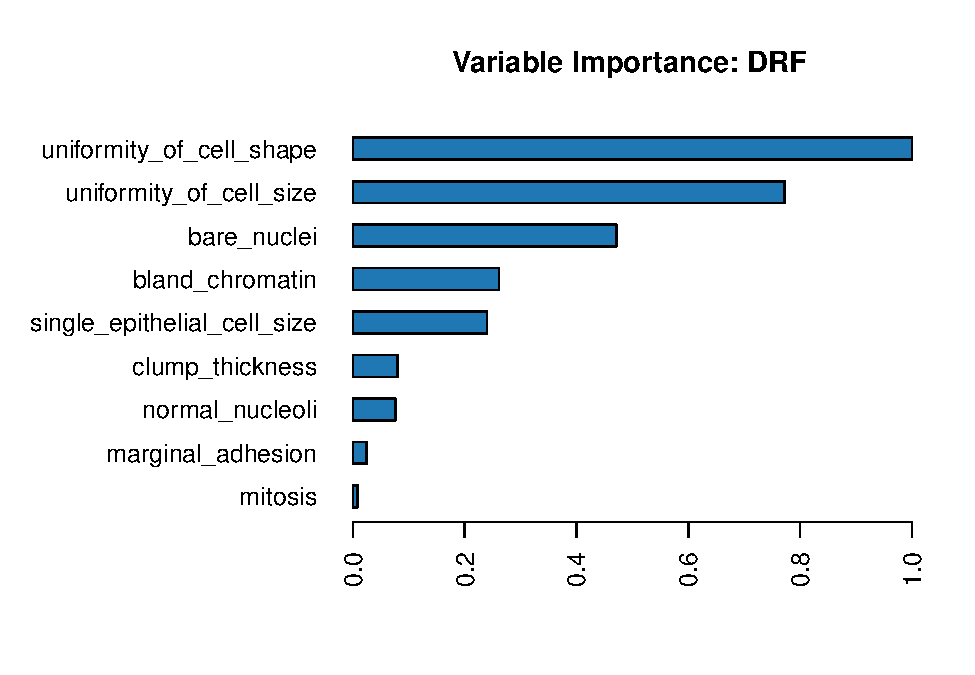
\includegraphics{webinar_code_files/figure-latex/unnamed-chunk-33-1.pdf}

\begin{Shaded}
\begin{Highlighting}[]
\CommentTok{#h2o.varimp(rf_model)}
\end{Highlighting}
\end{Shaded}

One performance metric we are interested in is the mean per class error
for training and validation data.

\begin{Shaded}
\begin{Highlighting}[]
\KeywordTok{h2o.mean_per_class_error}\NormalTok{(rf_model, }\DataTypeTok{train =} \OtherTok{TRUE}\NormalTok{, }\DataTypeTok{valid =} \OtherTok{TRUE}\NormalTok{, }\DataTypeTok{xval =} \OtherTok{TRUE}\NormalTok{)}
\end{Highlighting}
\end{Shaded}

\begin{verbatim}
##       train       valid        xval 
## 0.024674571 0.007042254 0.023097284
\end{verbatim}

The confusion matrix tells us, how many classes have been predicted
correctly and how many predictions were accurate. Here, we see the
errors in predictions on validation data

\begin{Shaded}
\begin{Highlighting}[]
\KeywordTok{h2o.confusionMatrix}\NormalTok{(rf_model, }\DataTypeTok{valid =} \OtherTok{TRUE}\NormalTok{)}
\end{Highlighting}
\end{Shaded}

\begin{verbatim}
## Confusion Matrix (vertical: actual; across: predicted)  for max f1 @ threshold = 0.293125896751881:
##           benign malignant    Error    Rate
## benign        70         1 0.014085   =1/71
## malignant      0        35 0.000000   =0/35
## Totals        70        36 0.009434  =1/106
\end{verbatim}

We can also plot the classification error.

\begin{Shaded}
\begin{Highlighting}[]
\KeywordTok{plot}\NormalTok{(rf_model,}
     \DataTypeTok{timestep =} \StringTok{"number_of_trees"}\NormalTok{,}
     \DataTypeTok{metric =} \StringTok{"classification_error"}\NormalTok{)}
\end{Highlighting}
\end{Shaded}

\begin{center}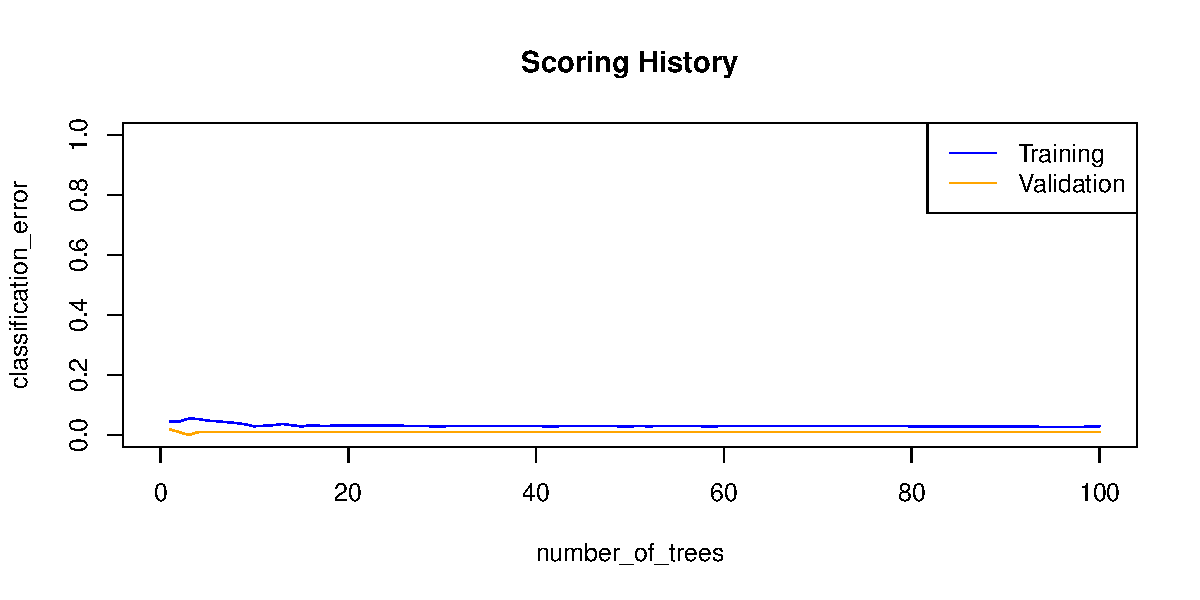
\includegraphics{webinar_code_files/figure-latex/unnamed-chunk-36-1} \end{center}

Next to the classification error, we are usually interested in the
logistic loss (negative log-likelihood or log loss). It describes the
sum of errors for each sample in the training or validation data or the
negative logarithm of the likelihood of error for a given prediction/
classification. Simply put, the lower the loss, the better the model (if
we ignore potential overfitting).

\begin{Shaded}
\begin{Highlighting}[]
\KeywordTok{plot}\NormalTok{(rf_model,}
     \DataTypeTok{timestep =} \StringTok{"number_of_trees"}\NormalTok{,}
     \DataTypeTok{metric =} \StringTok{"logloss"}\NormalTok{)}
\end{Highlighting}
\end{Shaded}

\begin{center}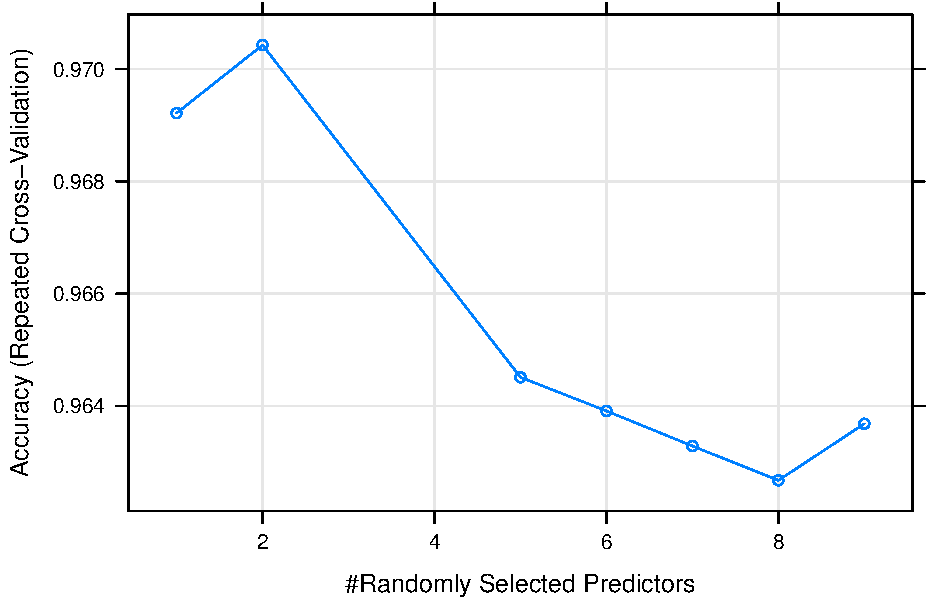
\includegraphics{webinar_code_files/figure-latex/unnamed-chunk-37-1} \end{center}

\begin{Shaded}
\begin{Highlighting}[]
\KeywordTok{plot}\NormalTok{(rf_model,}
     \DataTypeTok{timestep =} \StringTok{"number_of_trees"}\NormalTok{,}
     \DataTypeTok{metric =} \StringTok{"AUC"}\NormalTok{)}
\end{Highlighting}
\end{Shaded}

\begin{center}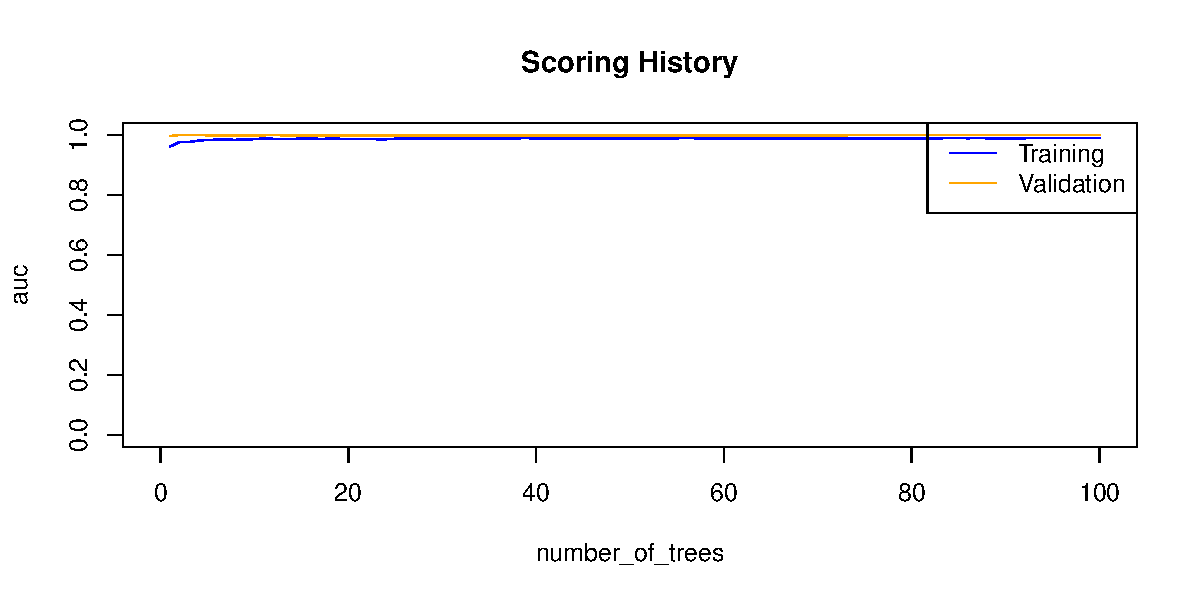
\includegraphics{webinar_code_files/figure-latex/unnamed-chunk-38-1} \end{center}

We can also plot the mean squared error (MSE). The MSE tells us the
average of the prediction errors squared, i.e.~the estimator's variance
and bias. The closer to zero, the better a model.

\begin{Shaded}
\begin{Highlighting}[]
\KeywordTok{plot}\NormalTok{(rf_model,}
     \DataTypeTok{timestep =} \StringTok{"number_of_trees"}\NormalTok{,}
     \DataTypeTok{metric =} \StringTok{"rmse"}\NormalTok{)}
\end{Highlighting}
\end{Shaded}

\begin{center}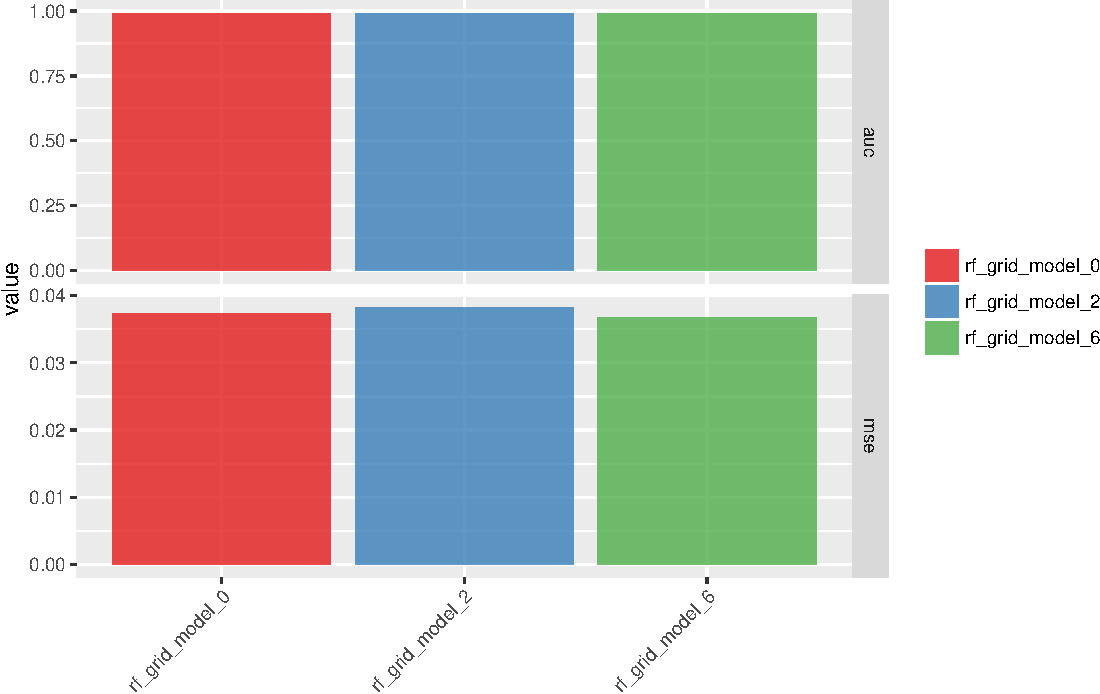
\includegraphics{webinar_code_files/figure-latex/unnamed-chunk-39-1} \end{center}

Next, we want to know the area under the curve (AUC). AUC is an
important metric for measuring binary classification model performances.
It gives the area under the curve, i.e.~the integral, of true positive
vs false positive rates. The closer to 1, the better a model. AUC is
especially useful, when we have unbalanced datasets (meaning datasets
where one class is much more common than the other), because it is
independent of class labels.

\begin{Shaded}
\begin{Highlighting}[]
\KeywordTok{h2o.auc}\NormalTok{(rf_model, }\DataTypeTok{train =} \OtherTok{TRUE}\NormalTok{)}
\end{Highlighting}
\end{Shaded}

\begin{verbatim}
## [1] 0.989521
\end{verbatim}

\begin{Shaded}
\begin{Highlighting}[]
\KeywordTok{h2o.auc}\NormalTok{(rf_model, }\DataTypeTok{valid =} \OtherTok{TRUE}\NormalTok{)}
\end{Highlighting}
\end{Shaded}

\begin{verbatim}
## [1] 0.9995976
\end{verbatim}

\begin{Shaded}
\begin{Highlighting}[]
\KeywordTok{h2o.auc}\NormalTok{(rf_model, }\DataTypeTok{xval =} \OtherTok{TRUE}\NormalTok{)}
\end{Highlighting}
\end{Shaded}

\begin{verbatim}
## [1] 0.9890496
\end{verbatim}

Now that we have a good idea about model performance on validation data,
we want to know how it performed on unseen test data. A good model
should find an optimal balance between accuracy on training and test
data. A model that has 0\% error on the training data but 40\% error on
the test data is in effect useless. It overfit on the training data and
is thus not able to generalize to unknown data.

\begin{Shaded}
\begin{Highlighting}[]
\NormalTok{perf <-}\StringTok{ }\KeywordTok{h2o.performance}\NormalTok{(rf_model, test)}
\NormalTok{perf}
\end{Highlighting}
\end{Shaded}

\begin{verbatim}
## H2OBinomialMetrics: drf
## 
## MSE:  0.03673598
## RMSE:  0.1916663
## LogLoss:  0.1158835
## Mean Per-Class Error:  0.0625
## AUC:  0.990625
## Gini:  0.98125
## 
## Confusion Matrix (vertical: actual; across: predicted) for F1-optimal threshold:
##           benign malignant    Error    Rate
## benign        70         0 0.000000   =0/70
## malignant      4        28 0.125000   =4/32
## Totals        74        28 0.039216  =4/102
## 
## Maximum Metrics: Maximum metrics at their respective thresholds
##                         metric threshold    value idx
## 1                       max f1  0.735027 0.933333  25
## 2                       max f2  0.294222 0.952381  37
## 3                 max f0point5  0.735027 0.972222  25
## 4                 max accuracy  0.735027 0.960784  25
## 5                max precision  1.000000 1.000000   0
## 6                   max recall  0.294222 1.000000  37
## 7              max specificity  1.000000 1.000000   0
## 8             max absolute_mcc  0.735027 0.909782  25
## 9   max min_per_class_accuracy  0.424524 0.937500  31
## 10 max mean_per_class_accuracy  0.294222 0.942857  37
## 
## Gains/Lift Table: Extract with `h2o.gainsLift(<model>, <data>)` or `h2o.gainsLift(<model>, valid=<T/F>, xval=<T/F>)`
\end{verbatim}

Plotting the test performance's AUC plot shows us approximately how good
the predictions are.

\begin{Shaded}
\begin{Highlighting}[]
\KeywordTok{plot}\NormalTok{(perf)}
\end{Highlighting}
\end{Shaded}

\begin{center}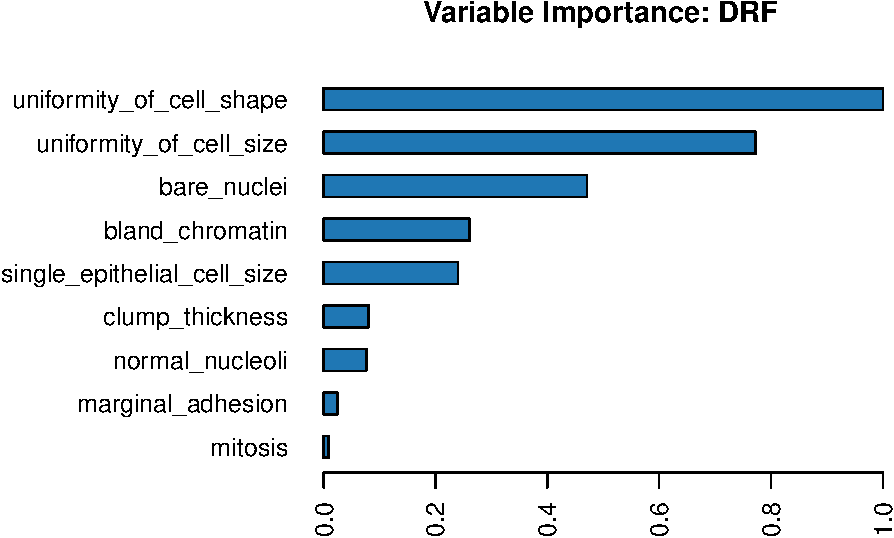
\includegraphics{webinar_code_files/figure-latex/unnamed-chunk-42-1} \end{center}

We also want to know the log loss, MSE and AUC values, as well as other
model metrics for the test data:

\begin{Shaded}
\begin{Highlighting}[]
\KeywordTok{h2o.logloss}\NormalTok{(perf)}
\end{Highlighting}
\end{Shaded}

\begin{verbatim}
## [1] 0.1158835
\end{verbatim}

\begin{Shaded}
\begin{Highlighting}[]
\KeywordTok{h2o.mse}\NormalTok{(perf)}
\end{Highlighting}
\end{Shaded}

\begin{verbatim}
## [1] 0.03673598
\end{verbatim}

\begin{Shaded}
\begin{Highlighting}[]
\KeywordTok{h2o.auc}\NormalTok{(perf)}
\end{Highlighting}
\end{Shaded}

\begin{verbatim}
## [1] 0.990625
\end{verbatim}

\begin{Shaded}
\begin{Highlighting}[]
\KeywordTok{head}\NormalTok{(}\KeywordTok{h2o.metric}\NormalTok{(perf))}
\end{Highlighting}
\end{Shaded}

\begin{verbatim}
## Metrics for Thresholds: Binomial metrics as a function of classification thresholds
##   threshold       f1       f2 f0point5 accuracy precision   recall
## 1  1.000000 0.171429 0.114504 0.340909 0.715686  1.000000 0.093750
## 2  0.998333 0.222222 0.151515 0.416667 0.725490  1.000000 0.125000
## 3  0.998000 0.270270 0.187970 0.480769 0.735294  1.000000 0.156250
## 4  0.997222 0.315789 0.223881 0.535714 0.745098  1.000000 0.187500
## 5  0.996210 0.358974 0.259259 0.583333 0.754902  1.000000 0.218750
## 6  0.994048 0.400000 0.294118 0.625000 0.764706  1.000000 0.250000
##   specificity absolute_mcc min_per_class_accuracy mean_per_class_accuracy
## 1    1.000000     0.257464               0.093750                0.546875
## 2    1.000000     0.298807               0.125000                0.562500
## 3    1.000000     0.335794               0.156250                0.578125
## 4    1.000000     0.369755               0.187500                0.593750
## 5    1.000000     0.401478               0.218750                0.609375
## 6    1.000000     0.431474               0.250000                0.625000
##   tns fns fps tps      tnr      fnr      fpr      tpr idx
## 1  70  29   0   3 1.000000 0.906250 0.000000 0.093750   0
## 2  70  28   0   4 1.000000 0.875000 0.000000 0.125000   1
## 3  70  27   0   5 1.000000 0.843750 0.000000 0.156250   2
## 4  70  26   0   6 1.000000 0.812500 0.000000 0.187500   3
## 5  70  25   0   7 1.000000 0.781250 0.000000 0.218750   4
## 6  70  24   0   8 1.000000 0.750000 0.000000 0.250000   5
\end{verbatim}

\subparagraph{Deep learning with neural
networks}\label{deep-learning-with-neural-networks}

\begin{Shaded}
\begin{Highlighting}[]
\NormalTok{hyper_params <-}\StringTok{ }\KeywordTok{list}\NormalTok{(}
                     \DataTypeTok{activation =} \KeywordTok{c}\NormalTok{(}\StringTok{"Rectifier"}\NormalTok{, }\StringTok{"Maxout"}\NormalTok{, }\StringTok{"Tanh"}\NormalTok{, }\StringTok{"RectifierWithDropout"}\NormalTok{, }
                                    \StringTok{"MaxoutWithDropout"}\NormalTok{, }\StringTok{"TanhWithDropout"}\NormalTok{), }
                     \DataTypeTok{hidden =} \KeywordTok{list}\NormalTok{(}\KeywordTok{c}\NormalTok{(}\DecValTok{5}\NormalTok{, }\DecValTok{5}\NormalTok{, }\DecValTok{5}\NormalTok{, }\DecValTok{5}\NormalTok{, }\DecValTok{5}\NormalTok{), }\KeywordTok{c}\NormalTok{(}\DecValTok{10}\NormalTok{, }\DecValTok{10}\NormalTok{, }\DecValTok{10}\NormalTok{, }\DecValTok{10}\NormalTok{), }\KeywordTok{c}\NormalTok{(}\DecValTok{50}\NormalTok{, }\DecValTok{50}\NormalTok{, }\DecValTok{50}\NormalTok{)),}
                     \DataTypeTok{epochs =} \KeywordTok{c}\NormalTok{(}\DecValTok{50}\NormalTok{, }\DecValTok{100}\NormalTok{, }\DecValTok{200}\NormalTok{),}
                     \DataTypeTok{l1 =} \KeywordTok{c}\NormalTok{(}\DecValTok{0}\NormalTok{, }\FloatTok{0.00001}\NormalTok{, }\FloatTok{0.0001}\NormalTok{), }
                     \DataTypeTok{l2 =} \KeywordTok{c}\NormalTok{(}\DecValTok{0}\NormalTok{, }\FloatTok{0.00001}\NormalTok{, }\FloatTok{0.0001}\NormalTok{),}
                     \DataTypeTok{rate =} \KeywordTok{c}\NormalTok{(}\DecValTok{0}\NormalTok{, }\DecValTok{01}\NormalTok{, }\FloatTok{0.005}\NormalTok{, }\FloatTok{0.001}\NormalTok{),}
                     \DataTypeTok{rate_annealing =} \KeywordTok{c}\NormalTok{(}\FloatTok{1e-8}\NormalTok{, }\FloatTok{1e-7}\NormalTok{, }\FloatTok{1e-6}\NormalTok{),}
                     \DataTypeTok{rho =} \KeywordTok{c}\NormalTok{(}\FloatTok{0.9}\NormalTok{,}\FloatTok{0.95}\NormalTok{,}\FloatTok{0.99}\NormalTok{,}\FloatTok{0.999}\NormalTok{),}
                     \DataTypeTok{epsilon =} \KeywordTok{c}\NormalTok{(}\FloatTok{1e-10}\NormalTok{,}\FloatTok{1e-8}\NormalTok{,}\FloatTok{1e-6}\NormalTok{,}\FloatTok{1e-4}\NormalTok{),}
                     \DataTypeTok{input_dropout_ratio =} \KeywordTok{c}\NormalTok{(}\DecValTok{0}\NormalTok{, }\FloatTok{0.1}\NormalTok{, }\FloatTok{0.2}\NormalTok{),}
                     \DataTypeTok{max_w2 =} \KeywordTok{c}\NormalTok{(}\DecValTok{10}\NormalTok{, }\DecValTok{100}\NormalTok{, }\DecValTok{1000}\NormalTok{, }\FloatTok{3.4028235e+38}\NormalTok{)}
                     \NormalTok{)}
\end{Highlighting}
\end{Shaded}

\begin{Shaded}
\begin{Highlighting}[]
\NormalTok{dl_grid <-}\StringTok{ }\KeywordTok{h2o.grid}\NormalTok{(}\DataTypeTok{algorithm =} \StringTok{"deeplearning"}\NormalTok{, }
                    \DataTypeTok{x =} \NormalTok{features,}
                    \DataTypeTok{y =} \NormalTok{response,}
                    \DataTypeTok{grid_id =} \StringTok{"dl_grid"}\NormalTok{,}
                    \DataTypeTok{training_frame =} \NormalTok{train,}
                    \DataTypeTok{validation_frame =} \NormalTok{valid,}
                    \DataTypeTok{nfolds =} \DecValTok{25}\NormalTok{,                           }
                    \DataTypeTok{fold_assignment =} \StringTok{"Stratified"}\NormalTok{,}
                    \DataTypeTok{hyper_params =} \NormalTok{hyper_params,}
                    \DataTypeTok{search_criteria =} \NormalTok{search_criteria,}
                    \DataTypeTok{seed =} \DecValTok{42}
                    \NormalTok{)}
\end{Highlighting}
\end{Shaded}

\begin{Shaded}
\begin{Highlighting}[]
\NormalTok{grid <-}\StringTok{ }\KeywordTok{h2o.getGrid}\NormalTok{(}\StringTok{"dl_grid"}\NormalTok{, }\DataTypeTok{sort_by =} \StringTok{"auc"}\NormalTok{, }\DataTypeTok{decreasing =} \OtherTok{TRUE}\NormalTok{)}
  
\NormalTok{model_ids <-}\StringTok{ }\NormalTok{grid@model_ids}
\NormalTok{best_model <-}\StringTok{ }\KeywordTok{h2o.getModel}\NormalTok{(model_ids[[}\DecValTok{1}\NormalTok{]])}
\end{Highlighting}
\end{Shaded}

Because training can take a while, depending on how many samples,
features, nodes and hidden layers you are training on, it is a good idea
to save your model.

\begin{Shaded}
\begin{Highlighting}[]
\KeywordTok{h2o.saveModel}\NormalTok{(best_model, }\DataTypeTok{path=}\StringTok{"models"}\NormalTok{, }\DataTypeTok{force =} \OtherTok{TRUE}\NormalTok{)}
\end{Highlighting}
\end{Shaded}

We can then re-load the model again any time to check the model quality
and make predictions on new data.

\begin{Shaded}
\begin{Highlighting}[]
\NormalTok{dl_model <-}\StringTok{ }\KeywordTok{h2o.loadModel}\NormalTok{(}\StringTok{"U:}\CharTok{\textbackslash{}\textbackslash{}}\StringTok{Github_blog}\CharTok{\textbackslash{}\textbackslash{}}\StringTok{Webinar}\CharTok{\textbackslash{}\textbackslash{}}\StringTok{Webinar_ML_for_disease}\CharTok{\textbackslash{}\textbackslash{}}\StringTok{models}\CharTok{\textbackslash{}\textbackslash{}}\StringTok{dl_grid_model_8"}\NormalTok{)}
\end{Highlighting}
\end{Shaded}

\begin{Shaded}
\begin{Highlighting}[]
\NormalTok{perf <-}\StringTok{ }\KeywordTok{h2o.performance}\NormalTok{(best_model, test)}
\KeywordTok{plot}\NormalTok{(perf)}
\end{Highlighting}
\end{Shaded}

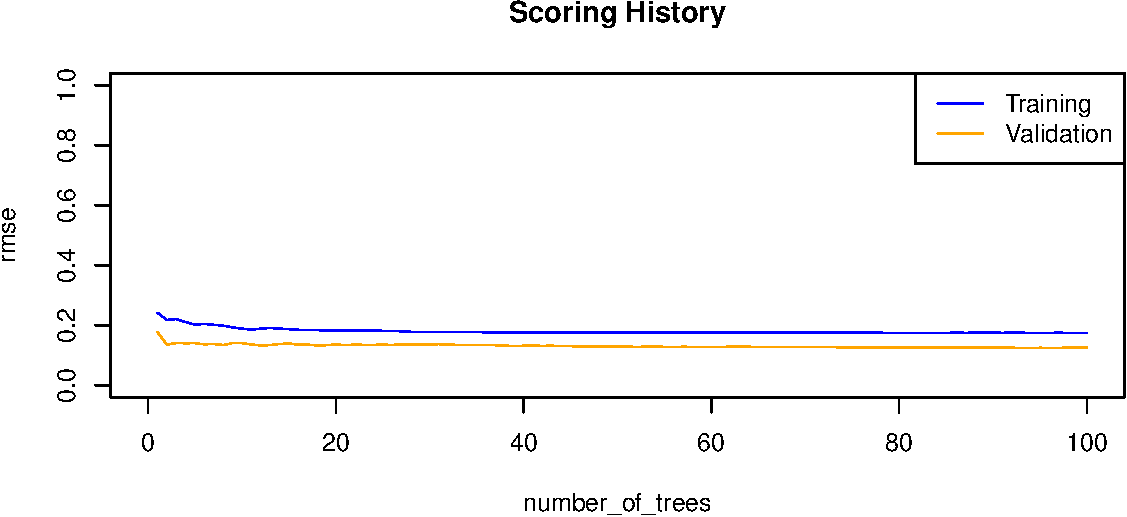
\includegraphics{webinar_code_files/figure-latex/unnamed-chunk-49-1.pdf}

\begin{Shaded}
\begin{Highlighting}[]
\KeywordTok{h2o.confusionMatrix}\NormalTok{(best_model, test)}
\end{Highlighting}
\end{Shaded}

\begin{verbatim}
## Confusion Matrix (vertical: actual; across: predicted)  for max f1 @ threshold = 0.735026690140367:
##           benign malignant    Error    Rate
## benign        70         0 0.000000   =0/70
## malignant      4        28 0.125000   =4/32
## Totals        74        28 0.039216  =4/102
\end{verbatim}

\begin{center}\rule{0.5\linewidth}{\linethickness}\end{center}

\subsection{Exercises}\label{exercises}

Try to run the analyses on the following datasets:

\subsubsection{Arrhythmia data}\label{arrhythmia-data}

The \href{https://archive.ics.uci.edu/ml/datasets/Arrhythmia}{arrhythmia
dataset} from the UC Irvine Machine Learning repository contains 279
features from ECG heart rhythm diagnostics and one output column. I am
not going to rename the feature columns because they are too many and
the descriptions are too complex. Also, we don't need to know
specifically which features we are looking at for building the models.
For a description of each feature, see
\url{https://archive.ics.uci.edu/ml/machine-learning-databases/arrhythmia/arrhythmia.names}.
The output column defines 16 classes: class 1 samples are from healthy
ECGs, the remaining classes belong to different types of arrhythmia,
with class 16 being all remaining arrhythmia cases that didn't fit into
distinct classes.

\begin{Shaded}
\begin{Highlighting}[]
\NormalTok{arrhythmia <-}\StringTok{ }\KeywordTok{read.table}\NormalTok{(}\StringTok{"datasets/arrhythmia.data.txt"}\NormalTok{, }\DataTypeTok{sep =} \StringTok{","}\NormalTok{)}
\NormalTok{arrhythmia[arrhythmia ==}\StringTok{ "?"}\NormalTok{] <-}\StringTok{ }\OtherTok{NA}

\CommentTok{# making sure, that all feature columns are numeric}
\NormalTok{arrhythmia[-}\DecValTok{280}\NormalTok{] <-}\StringTok{ }\KeywordTok{lapply}\NormalTok{(arrhythmia[-}\DecValTok{280}\NormalTok{], as.character)}
\NormalTok{arrhythmia[-}\DecValTok{280}\NormalTok{] <-}\StringTok{ }\KeywordTok{lapply}\NormalTok{(arrhythmia[-}\DecValTok{280}\NormalTok{], as.numeric)}

\CommentTok{#  renaming output column and converting to factor}
\KeywordTok{colnames}\NormalTok{(arrhythmia)[}\DecValTok{280}\NormalTok{] <-}\StringTok{ "class"}
\NormalTok{arrhythmia$class <-}\StringTok{ }\KeywordTok{as.factor}\NormalTok{(arrhythmia$class)}

\NormalTok{arrhythmia$diagnosis <-}\StringTok{ }\KeywordTok{ifelse}\NormalTok{(arrhythmia$class ==}\StringTok{ }\DecValTok{1}\NormalTok{, }\StringTok{"healthy"}\NormalTok{, }\StringTok{"arrhythmia"}\NormalTok{)}
\NormalTok{arrhythmia$diagnosis <-}\StringTok{ }\KeywordTok{as.factor}\NormalTok{(arrhythmia$diagnosis)}
\end{Highlighting}
\end{Shaded}

\subsubsection{Flu data}\label{flu-data}

Among the many R packages, there is the
\href{https://mran.microsoft.com/web/packages/outbreaks/outbreaks.pdf}{outbreaks}
package. It contains datasets on epidemics, on of which is from the 2013
outbreak of
\href{http://www.who.int/influenza/human_animal_interface/faq_H7N9/en/}{influenza
A H7N9} in
\href{http://www.who.int/influenza/human_animal_interface/influenza_h7n9/ChinaH7N9JointMissionReport2013u.pdf?ua=1}{China},
as analysed by Kucharski et al. (2014):

\begin{Shaded}
\begin{Highlighting}[]
\KeywordTok{library}\NormalTok{(outbreaks)}
\KeywordTok{data}\NormalTok{(fluH7N9_china_2013)}

\CommentTok{# convert ? to NAs}
\NormalTok{fluH7N9_china_2013$age[}\KeywordTok{which}\NormalTok{(fluH7N9_china_2013$age ==}\StringTok{ "?"}\NormalTok{)] <-}\StringTok{ }\OtherTok{NA}

\CommentTok{# create a new column with case ID}
\NormalTok{fluH7N9_china_2013$case.ID <-}\StringTok{ }\KeywordTok{paste}\NormalTok{(}\StringTok{"case"}\NormalTok{, fluH7N9_china_2013$case.ID, }\DataTypeTok{sep =} \StringTok{"_"}\NormalTok{)}

\CommentTok{# preparing the data frame for modeling}
\CommentTok{# }
\KeywordTok{library}\NormalTok{(dplyr)}

\NormalTok{dataset <-}\StringTok{ }\NormalTok{fluH7N9_china_2013 %>%}
\StringTok{  }\KeywordTok{mutate}\NormalTok{(}\DataTypeTok{hospital =} \KeywordTok{as.factor}\NormalTok{(}\KeywordTok{ifelse}\NormalTok{(}\KeywordTok{is.na}\NormalTok{(date_of_hospitalisation), }\DecValTok{0}\NormalTok{, }\DecValTok{1}\NormalTok{)),}
         \DataTypeTok{gender_f =} \KeywordTok{as.factor}\NormalTok{(}\KeywordTok{ifelse}\NormalTok{(gender ==}\StringTok{ "f"}\NormalTok{, }\DecValTok{1}\NormalTok{, }\DecValTok{0}\NormalTok{)),}
         \DataTypeTok{province_Jiangsu =} \KeywordTok{as.factor}\NormalTok{(}\KeywordTok{ifelse}\NormalTok{(province ==}\StringTok{ "Jiangsu"}\NormalTok{, }\DecValTok{1}\NormalTok{, }\DecValTok{0}\NormalTok{)),}
         \DataTypeTok{province_Shanghai =} \KeywordTok{as.factor}\NormalTok{(}\KeywordTok{ifelse}\NormalTok{(province ==}\StringTok{ "Shanghai"}\NormalTok{, }\DecValTok{1}\NormalTok{, }\DecValTok{0}\NormalTok{)),}
         \DataTypeTok{province_Zhejiang =} \KeywordTok{as.factor}\NormalTok{(}\KeywordTok{ifelse}\NormalTok{(province ==}\StringTok{ "Zhejiang"}\NormalTok{, }\DecValTok{1}\NormalTok{, }\DecValTok{0}\NormalTok{)),}
         \DataTypeTok{province_other =} \KeywordTok{as.factor}\NormalTok{(}\KeywordTok{ifelse}\NormalTok{(province ==}\StringTok{ "Zhejiang"} \NormalTok{|}\StringTok{ }\NormalTok{province ==}\StringTok{ "Jiangsu"} \NormalTok{|}\StringTok{ }\NormalTok{province ==}\StringTok{ "Shanghai"}\NormalTok{, }\DecValTok{0}\NormalTok{, }\DecValTok{1}\NormalTok{)),}
         \DataTypeTok{days_onset_to_outcome =} \KeywordTok{as.numeric}\NormalTok{(}\KeywordTok{as.character}\NormalTok{(}\KeywordTok{gsub}\NormalTok{(}\StringTok{" days"}\NormalTok{, }\StringTok{""}\NormalTok{,}
                                      \KeywordTok{as.Date}\NormalTok{(}\KeywordTok{as.character}\NormalTok{(date_of_outcome), }\DataTypeTok{format =} \StringTok{"%Y-%m-%d"}\NormalTok{) -}\StringTok{ }
\StringTok{                                        }\KeywordTok{as.Date}\NormalTok{(}\KeywordTok{as.character}\NormalTok{(date_of_onset), }\DataTypeTok{format =} \StringTok{"%Y-%m-%d"}\NormalTok{)))),}
         \DataTypeTok{days_onset_to_hospital =} \KeywordTok{as.numeric}\NormalTok{(}\KeywordTok{as.character}\NormalTok{(}\KeywordTok{gsub}\NormalTok{(}\StringTok{" days"}\NormalTok{, }\StringTok{""}\NormalTok{,}
                                      \KeywordTok{as.Date}\NormalTok{(}\KeywordTok{as.character}\NormalTok{(date_of_hospitalisation), }\DataTypeTok{format =} \StringTok{"%Y-%m-%d"}\NormalTok{) -}\StringTok{ }
\StringTok{                                        }\KeywordTok{as.Date}\NormalTok{(}\KeywordTok{as.character}\NormalTok{(date_of_onset), }\DataTypeTok{format =} \StringTok{"%Y-%m-%d"}\NormalTok{)))),}
         \DataTypeTok{age =} \KeywordTok{as.numeric}\NormalTok{(}\KeywordTok{as.character}\NormalTok{(age)),}
         \DataTypeTok{early_onset =} \KeywordTok{as.factor}\NormalTok{(}\KeywordTok{ifelse}\NormalTok{(date_of_onset <}\StringTok{ }\KeywordTok{summary}\NormalTok{(fluH7N9_china_2013$date_of_onset)[[}\DecValTok{3}\NormalTok{]], }\DecValTok{1}\NormalTok{, }\DecValTok{0}\NormalTok{)),}
         \DataTypeTok{early_outcome =} \KeywordTok{as.factor}\NormalTok{(}\KeywordTok{ifelse}\NormalTok{(date_of_outcome <}\StringTok{ }\KeywordTok{summary}\NormalTok{(fluH7N9_china_2013$date_of_outcome)[[}\DecValTok{3}\NormalTok{]], }\DecValTok{1}\NormalTok{, }\DecValTok{0}\NormalTok{))) %>%}
\StringTok{  }\KeywordTok{subset}\NormalTok{(}\DataTypeTok{select =} \NormalTok{-}\KeywordTok{c}\NormalTok{(}\DecValTok{2}\NormalTok{:}\DecValTok{4}\NormalTok{, }\DecValTok{6}\NormalTok{, }\DecValTok{8}\NormalTok{))}
\KeywordTok{rownames}\NormalTok{(dataset) <-}\StringTok{ }\NormalTok{dataset$case_id}
\NormalTok{dataset <-}\StringTok{ }\NormalTok{dataset[, -}\DecValTok{1}\NormalTok{]}

\CommentTok{# impute missing data}

\KeywordTok{library}\NormalTok{(mice)}
\end{Highlighting}
\end{Shaded}

\begin{verbatim}
## 
## Attaching package: 'mice'
\end{verbatim}

\begin{verbatim}
## The following object is masked from 'package:tidyr':
## 
##     complete
\end{verbatim}

\begin{Shaded}
\begin{Highlighting}[]
\NormalTok{dataset_impute <-}\StringTok{ }\KeywordTok{mice}\NormalTok{(dataset[, -}\DecValTok{1}\NormalTok{],  }\DataTypeTok{print =} \OtherTok{FALSE}\NormalTok{)}

\CommentTok{# recombine imputed data frame with the outcome column}

\NormalTok{dataset_complete <-}\StringTok{ }\KeywordTok{merge}\NormalTok{(dataset[, }\DecValTok{1}\NormalTok{, }\DataTypeTok{drop =} \OtherTok{FALSE}\NormalTok{], mice::}\KeywordTok{complete}\NormalTok{(dataset_impute, }\DecValTok{1}\NormalTok{), }\DataTypeTok{by =} \StringTok{"row.names"}\NormalTok{, }\DataTypeTok{all =} \OtherTok{TRUE}\NormalTok{)}
\KeywordTok{rownames}\NormalTok{(dataset_complete) <-}\StringTok{ }\NormalTok{dataset_complete$Row.names}
\NormalTok{dataset_complete <-}\StringTok{ }\NormalTok{dataset_complete[, -}\DecValTok{1}\NormalTok{]}
\end{Highlighting}
\end{Shaded}

\begin{center}\rule{0.5\linewidth}{\linethickness}\end{center}

\begin{Shaded}
\begin{Highlighting}[]
\KeywordTok{sessionInfo}\NormalTok{()}
\end{Highlighting}
\end{Shaded}

\begin{verbatim}
## R version 3.3.2 (2016-10-31)
## Platform: x86_64-w64-mingw32/x64 (64-bit)
## Running under: Windows 7 x64 (build 7601) Service Pack 1
## 
## locale:
## [1] LC_COLLATE=English_United States.1252 
## [2] LC_CTYPE=English_United States.1252   
## [3] LC_MONETARY=English_United States.1252
## [4] LC_NUMERIC=C                          
## [5] LC_TIME=English_United States.1252    
## 
## attached base packages:
## [1] stats     graphics  grDevices utils     datasets  methods   base     
## 
## other attached packages:
##  [1] mice_2.30           outbreaks_1.2.0     h2o_3.10.3.6       
##  [4] plyr_1.8.4          xgboost_0.6-4       randomForest_4.6-12
##  [7] rpart.plot_2.1.1    rpart_4.1-10        tidyr_0.6.1        
## [10] dplyr_0.5.0         caret_6.0-73        ggplot2_2.2.1.9000 
## [13] lattice_0.20-34    
## 
## loaded via a namespace (and not attached):
##  [1] reshape2_1.4.2     splines_3.3.2      colorspace_1.3-2  
##  [4] htmltools_0.3.5    stats4_3.3.2       yaml_2.1.14       
##  [7] mgcv_1.8-17        survival_2.40-1    ModelMetrics_1.1.0
## [10] e1071_1.6-8        nloptr_1.0.4       DBI_0.5-1         
## [13] RColorBrewer_1.1-2 foreach_1.4.3      stringr_1.2.0     
## [16] MatrixModels_0.4-1 munsell_0.4.3      gtable_0.2.0      
## [19] codetools_0.2-15   evaluate_0.10      labeling_0.3      
## [22] knitr_1.15.1       SparseM_1.74       quantreg_5.29     
## [25] pbkrtest_0.4-6     parallel_3.3.2     class_7.3-14      
## [28] Rcpp_0.12.9        scales_0.4.1       backports_1.0.5   
## [31] jsonlite_1.3       lme4_1.1-12        digest_0.6.12     
## [34] stringi_1.1.2      grid_3.3.2         rprojroot_1.2     
## [37] tools_3.3.2        bitops_1.0-6       magrittr_1.5      
## [40] lazyeval_0.2.0     RCurl_1.95-4.8     tibble_1.2        
## [43] car_2.1-4          MASS_7.3-45        Matrix_1.2-8      
## [46] data.table_1.10.4  assertthat_0.1     minqa_1.2.4       
## [49] rmarkdown_1.3      iterators_1.0.8    R6_2.2.0          
## [52] nnet_7.3-12        nlme_3.1-131
\end{verbatim}


\end{document}
